\documentclass{beamer}	
\mode<presentation>
 
\usepackage{pdfpages}
\usepackage{fancyvrb}
\usepackage{chemarr}

\usepackage{amsmath}		%% mathematics typesetting
\usepackage{amssymb}
 
\usepackage{ulem}

\usepackage{booktabs}

\usepackage{siunitx} %% tpyeset SI units

\usepackage{CJKutf8} %% typeset Chinese characters

\usepackage{pdfpages}

% Color and Theme. Can be changed. However, this one's quite nice.
\usetheme{Madrid}
\definecolor{theme}{rgb}{0.84,0,0.21}
\usecolortheme[named=theme]{structure}


%%  Title information
\title[M01.2 Mechanik]{M01.2 Mechanik}
\author[melanie.stefan@medicalschool-berlin.de]{M01 Physik für Mediziner*innen}
\institute[]{Prof. Melanie Stefan - melanie.stefan@medcialschool-berlin.de}
\date{WiSe 2022/23}
 

% Table of contents to pop up at the beginning of each section
\AtBeginSection[]
{
  \begin{frame}<beamer>
    \frametitle{Outline}
    \tableofcontents[currentsection,currentsubsection]
  \end{frame}
}
 
\beamertemplatenavigationsymbolsempty

\begin{document}
 


 { \usebackgroundtemplate{
\includegraphics[width=1.2\paperwidth]{MSB_Titelseite.pdf}} 
\begin{frame}

 \maketitle 

$\,$\\[6cm] 


\end{frame} 
}
 


%% Hook
\begin{frame}
\frametitle{Neulich auf  olympics.com \dots}

\begin{center}
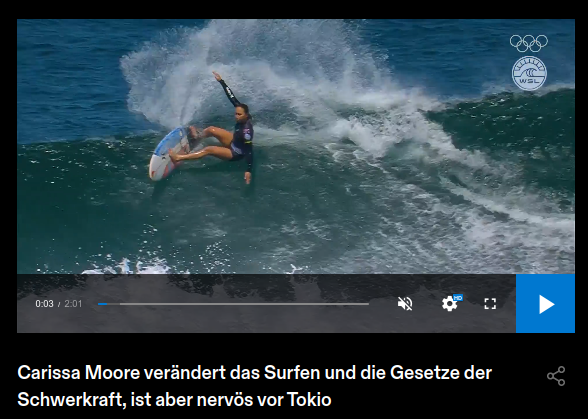
\includegraphics[width=0.9\textwidth]{surfen_schwerkraft.png}
\end{center}

 
\end{frame}

%% TLIA
\begin{frame}
\frametitle{In dieser Vorlesung geht es um \dots}

Bewegung und Verformung von Körpern und damit einhergehende Kräfte

\begin{center}
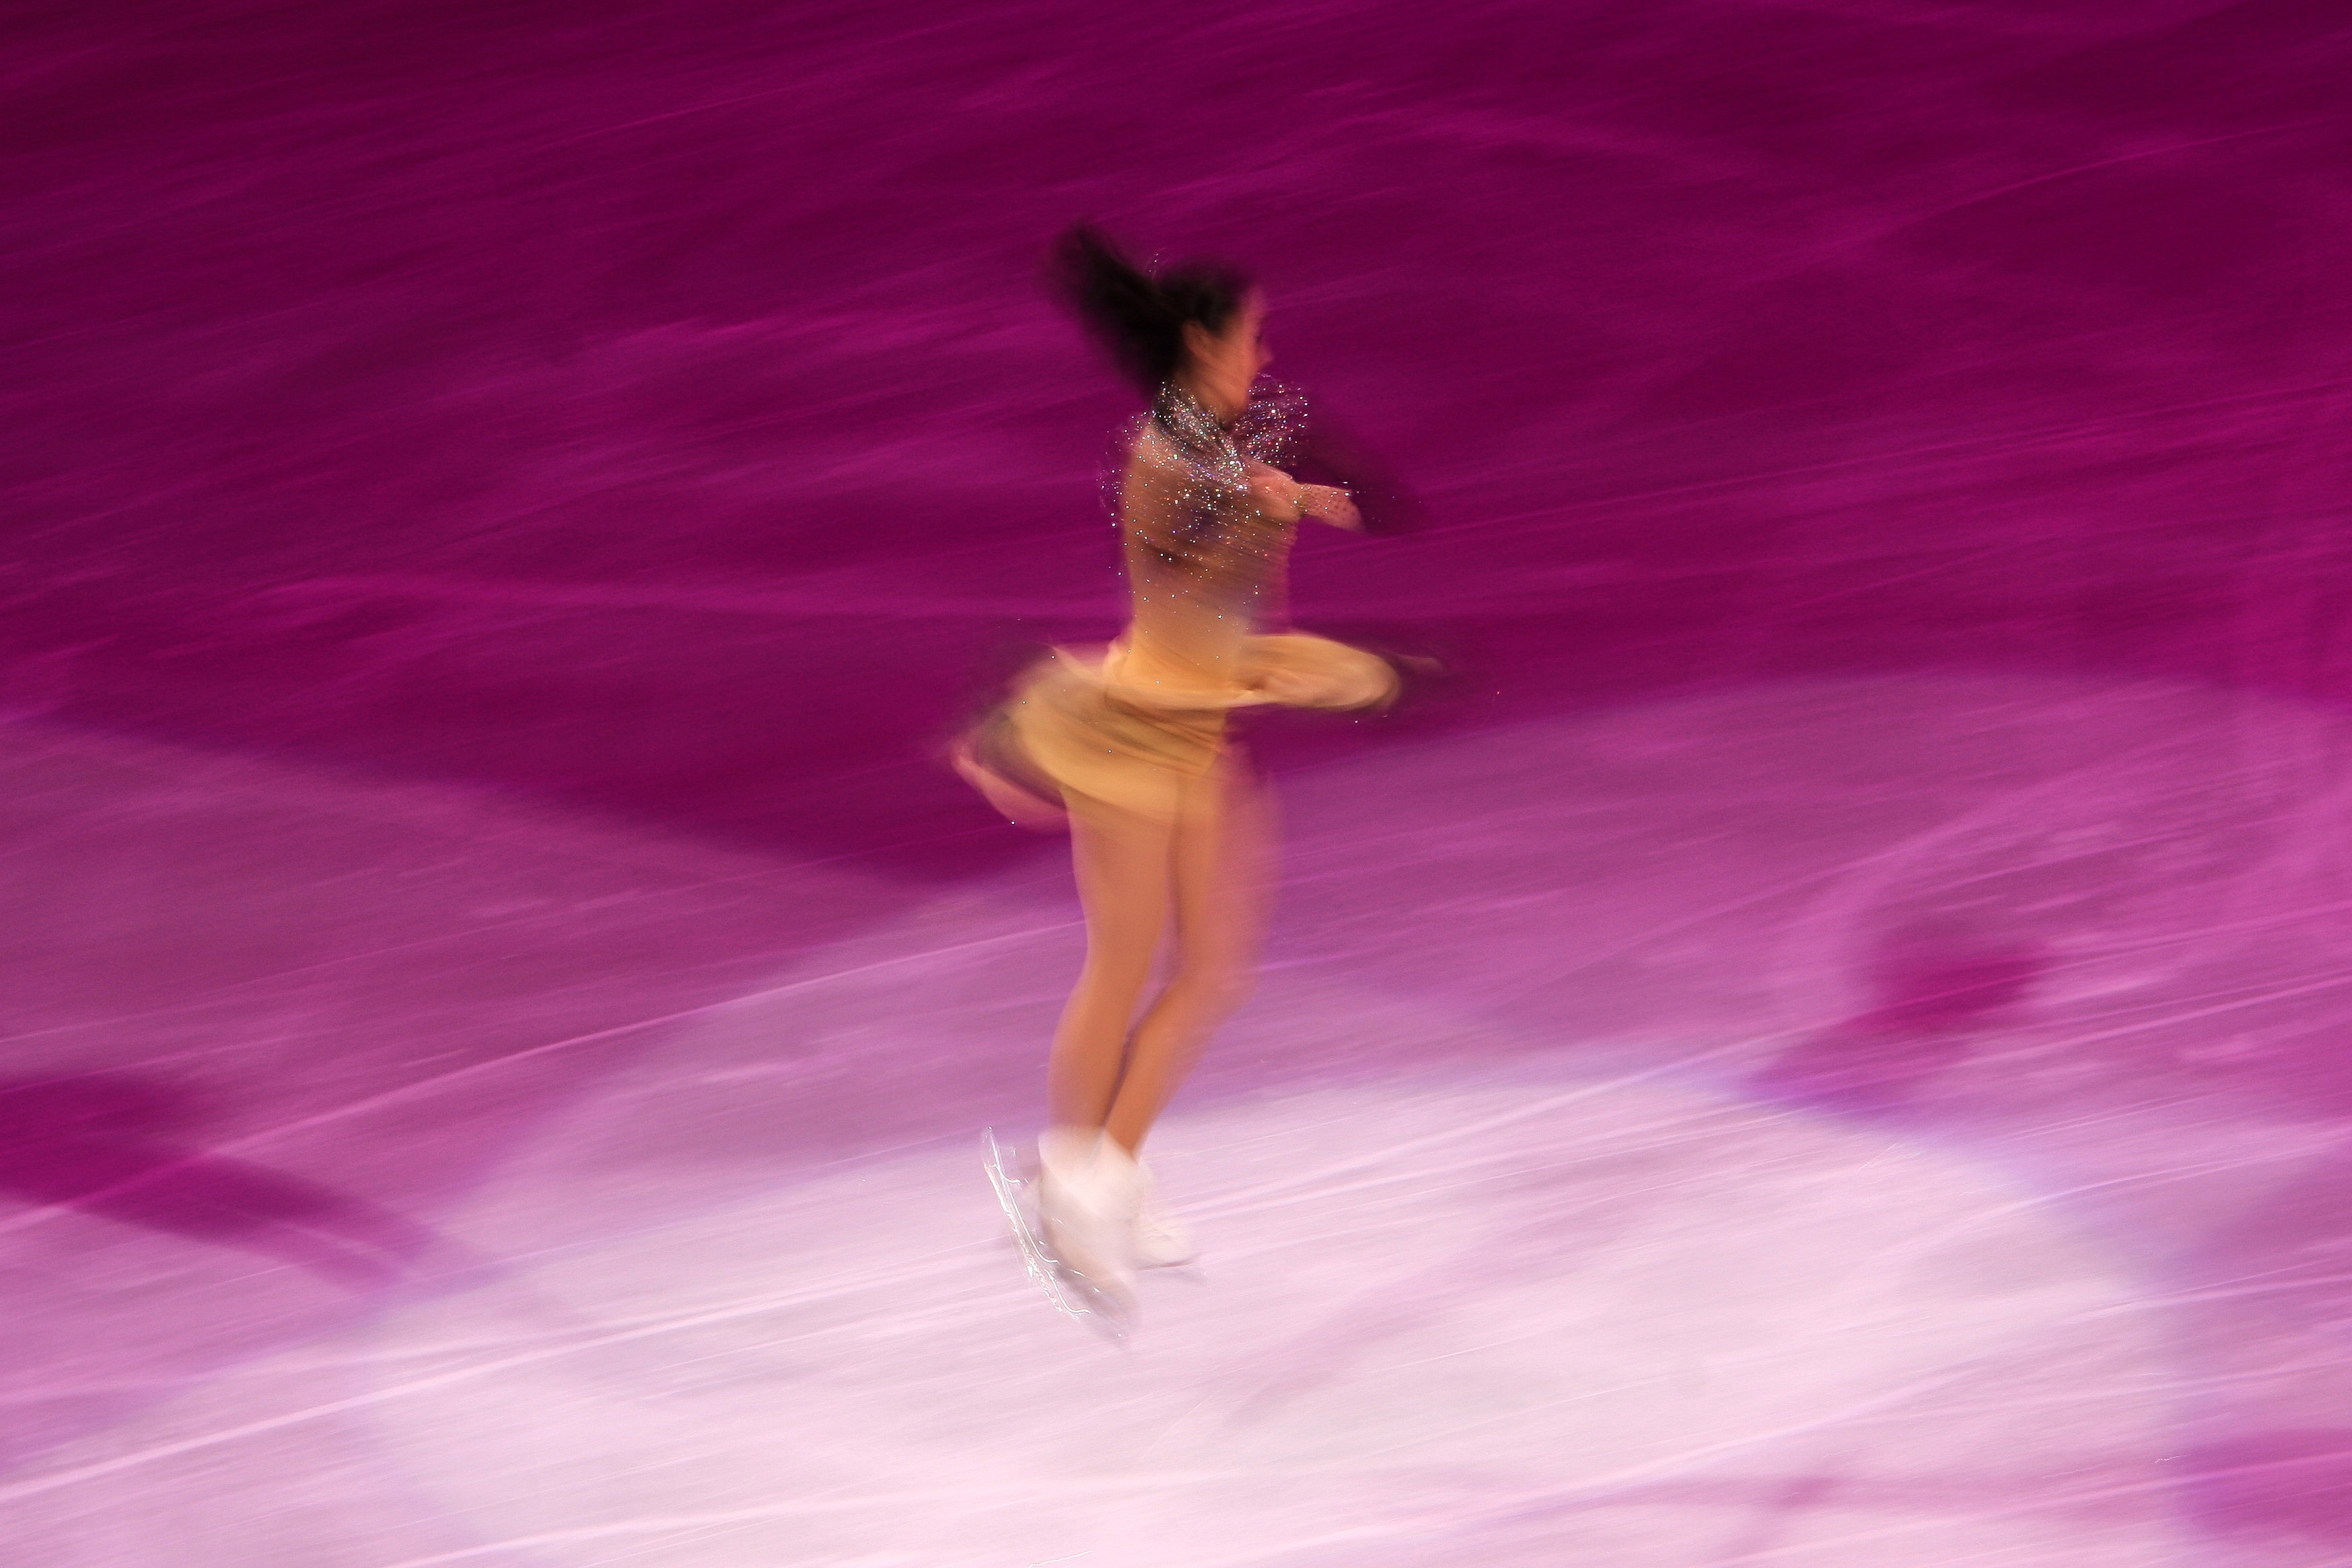
\includegraphics[width=0.9\textwidth]{figureskater.jpg}
\end{center}

 
\end{frame}



%% Learning Objectives
 
\begin{frame}

\frametitle{Nach dieser Vorlesung sollten Sie:}



\begin{block}{Wissen:}
\begin{itemize}
\item
Zusammenhang zwischen Strecke, Geschwindigkeit und Beschleunigung erklären
\item
Periodendauer, Frequenz und Kreisfrequenz definieren
\item
die Newtonschen Axiome nennen
\item
Impuls und Kraft definieren
\item
den  Impulserhaltungssatz wiedergeben und Beispiele geben
\item
Arbeit, Leistung und Energie definieren
\item
Arten von Energie unterscheiden
\item
den Energieerhaltungssatz erklären
\item
Drehmoment definieren und das Hebelgesetz
\item
Trägheitsmoment und Drehimpuls definieren
\item
den Drehimpulserhaltungssatz erklären und Beispiele nennen 
\end{itemize}

\end{block}

\end{frame}

\begin{frame}

\frametitle{Nach dieser Vorlesung sollten Sie:}
 



\begin{block}{Können:}
\begin{itemize}
\item
Bewegungsdiagramme lesen und verstehen/auswerten
\item
Mittelwert und Momentanwert der Geschwindigkeit errechnen
\item
Parameter einer Kreisbewegung berechnen
\item 
das Hebelgesetz anwenden
\end{itemize}
\end{block}


 
\begin{block}{Fühlen:}
\begin{itemize}
\item
mechanische Prozesse im täglichen Leben erkennen
\item
über Anwendungen von Mechanik in der Medizin nachdenken
\end{itemize}
\end{block}

 \end{frame}


%% Main Body

\section{Bewegungen} 


\begin{frame}
\makebox[\linewidth]{\includegraphics[page=3,width=\textwidth]{Walter_Mechanik.pdf}}
\end{frame}

\begin{frame}
\makebox[\linewidth]{\includegraphics[page=4,width=\textwidth]{Walter_Mechanik.pdf}}
\end{frame}

\begin{frame}
\makebox[\linewidth]{\includegraphics[page=5,width=\textwidth]{Walter_Mechanik.pdf}}
\end{frame}



\begin{frame}
\makebox[\linewidth]{\includegraphics[page=6,width=\textwidth]{Walter_Mechanik.pdf}}
\end{frame}
\begin{frame}
\makebox[\linewidth]{\includegraphics[page=7,width=\textwidth]{Walter_Mechanik.pdf}}
\end{frame}

\begin{frame}
\makebox[\linewidth]{\includegraphics[page=8,width=\textwidth]{Walter_Mechanik.pdf}}
\end{frame}

\begin{frame}
\makebox[\linewidth]{\includegraphics[page=9,width=\textwidth]{Walter_Mechanik.pdf}}
\end{frame}

\begin{frame}
\makebox[\linewidth]{\includegraphics[page=10,width=\textwidth]{Walter_Mechanik.pdf}}
\end{frame}



\begin{frame}
\makebox[\linewidth]{\includegraphics[page=11,width=\textwidth]{Walter_Mechanik.pdf}}
\end{frame}




%% # periodische Bewegungen,
%% # Definition und Einheit von Periodendauer,
%% # Frequenz und Kreisfrequenz

\begin{frame}
\frametitle{Kreisbewegung}

Wie schnell dreht sich ein Rad?

\begin{center}
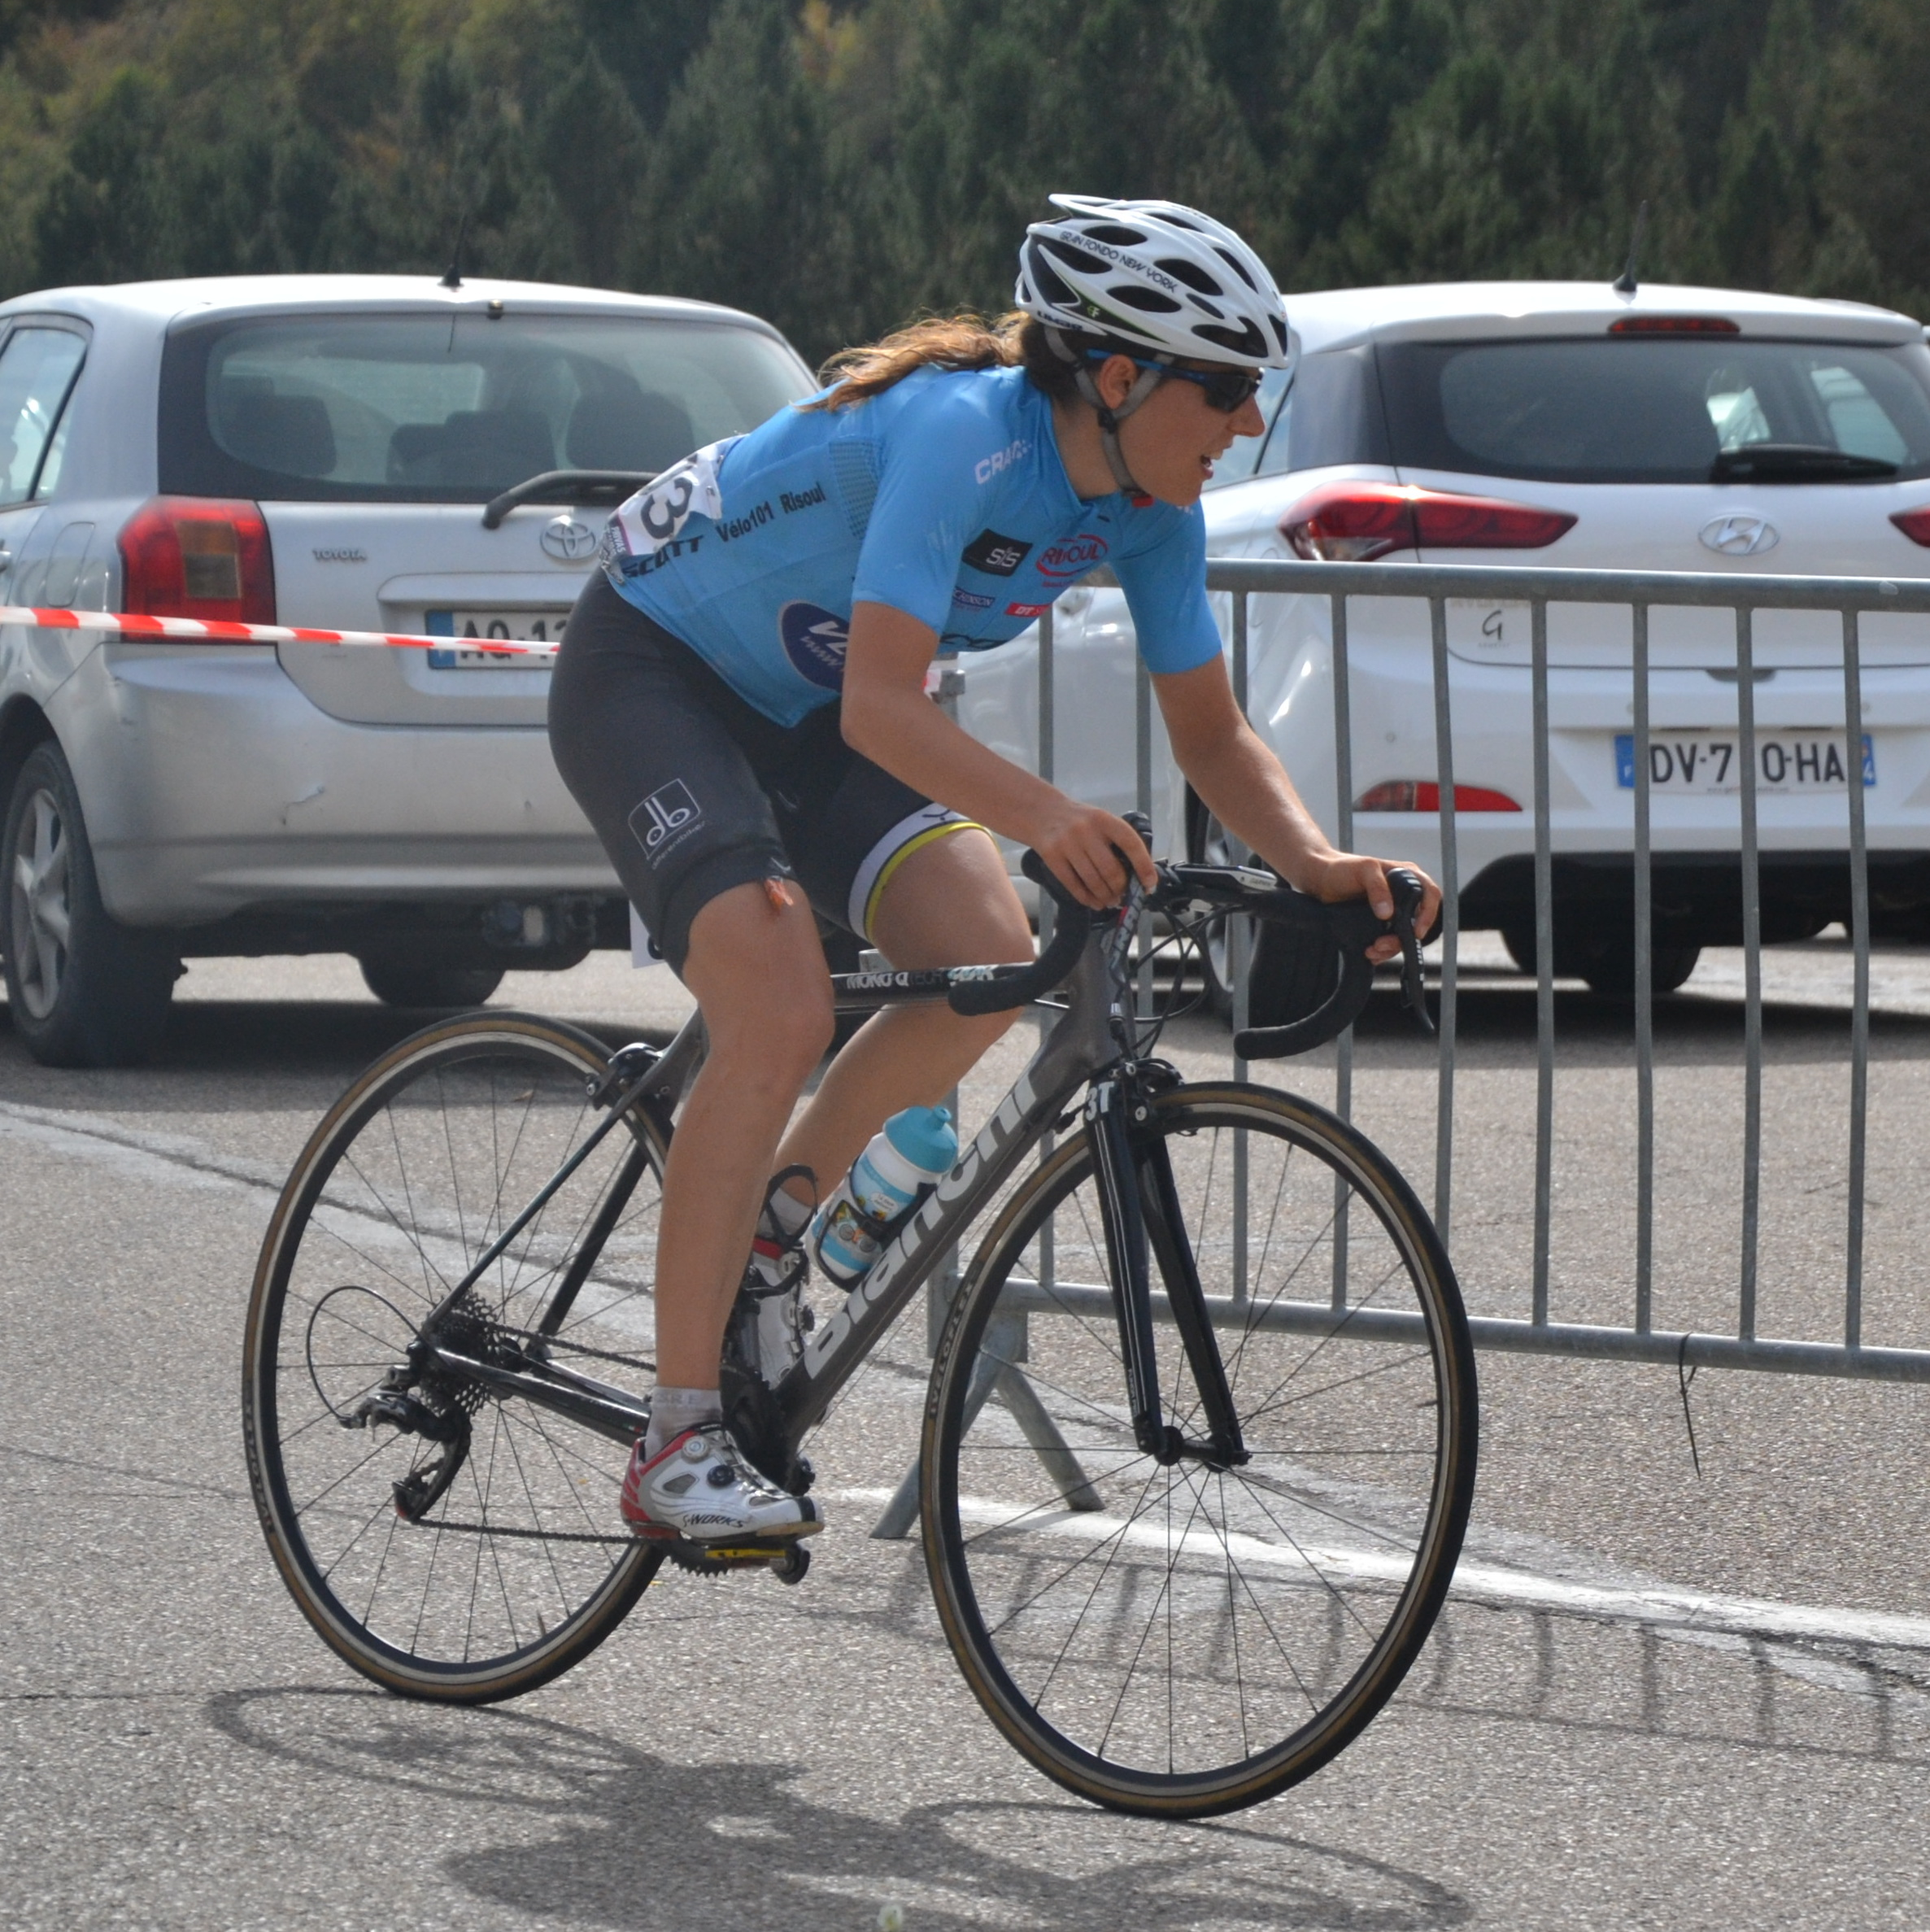
\includegraphics[width=0.7\textwidth]{fahrrad.jpg}
\end{center}

\end{frame}


\begin{frame}
\frametitle{Kreisbewegung}

Die Geschwindigkeit einer Kreisbewegung kann unterschiedlich definiert werden


\begin{columns}[c]

\begin{column}{8cm}

\begin{itemize}
\item
Frequenz f: Umdrehungen pro Sekunde. \\
Einheit: s$^{-1}$ =  Hz (Hertz) \\

\end{itemize}

\end{column}

\begin{column}{3cm}
\begin{center}
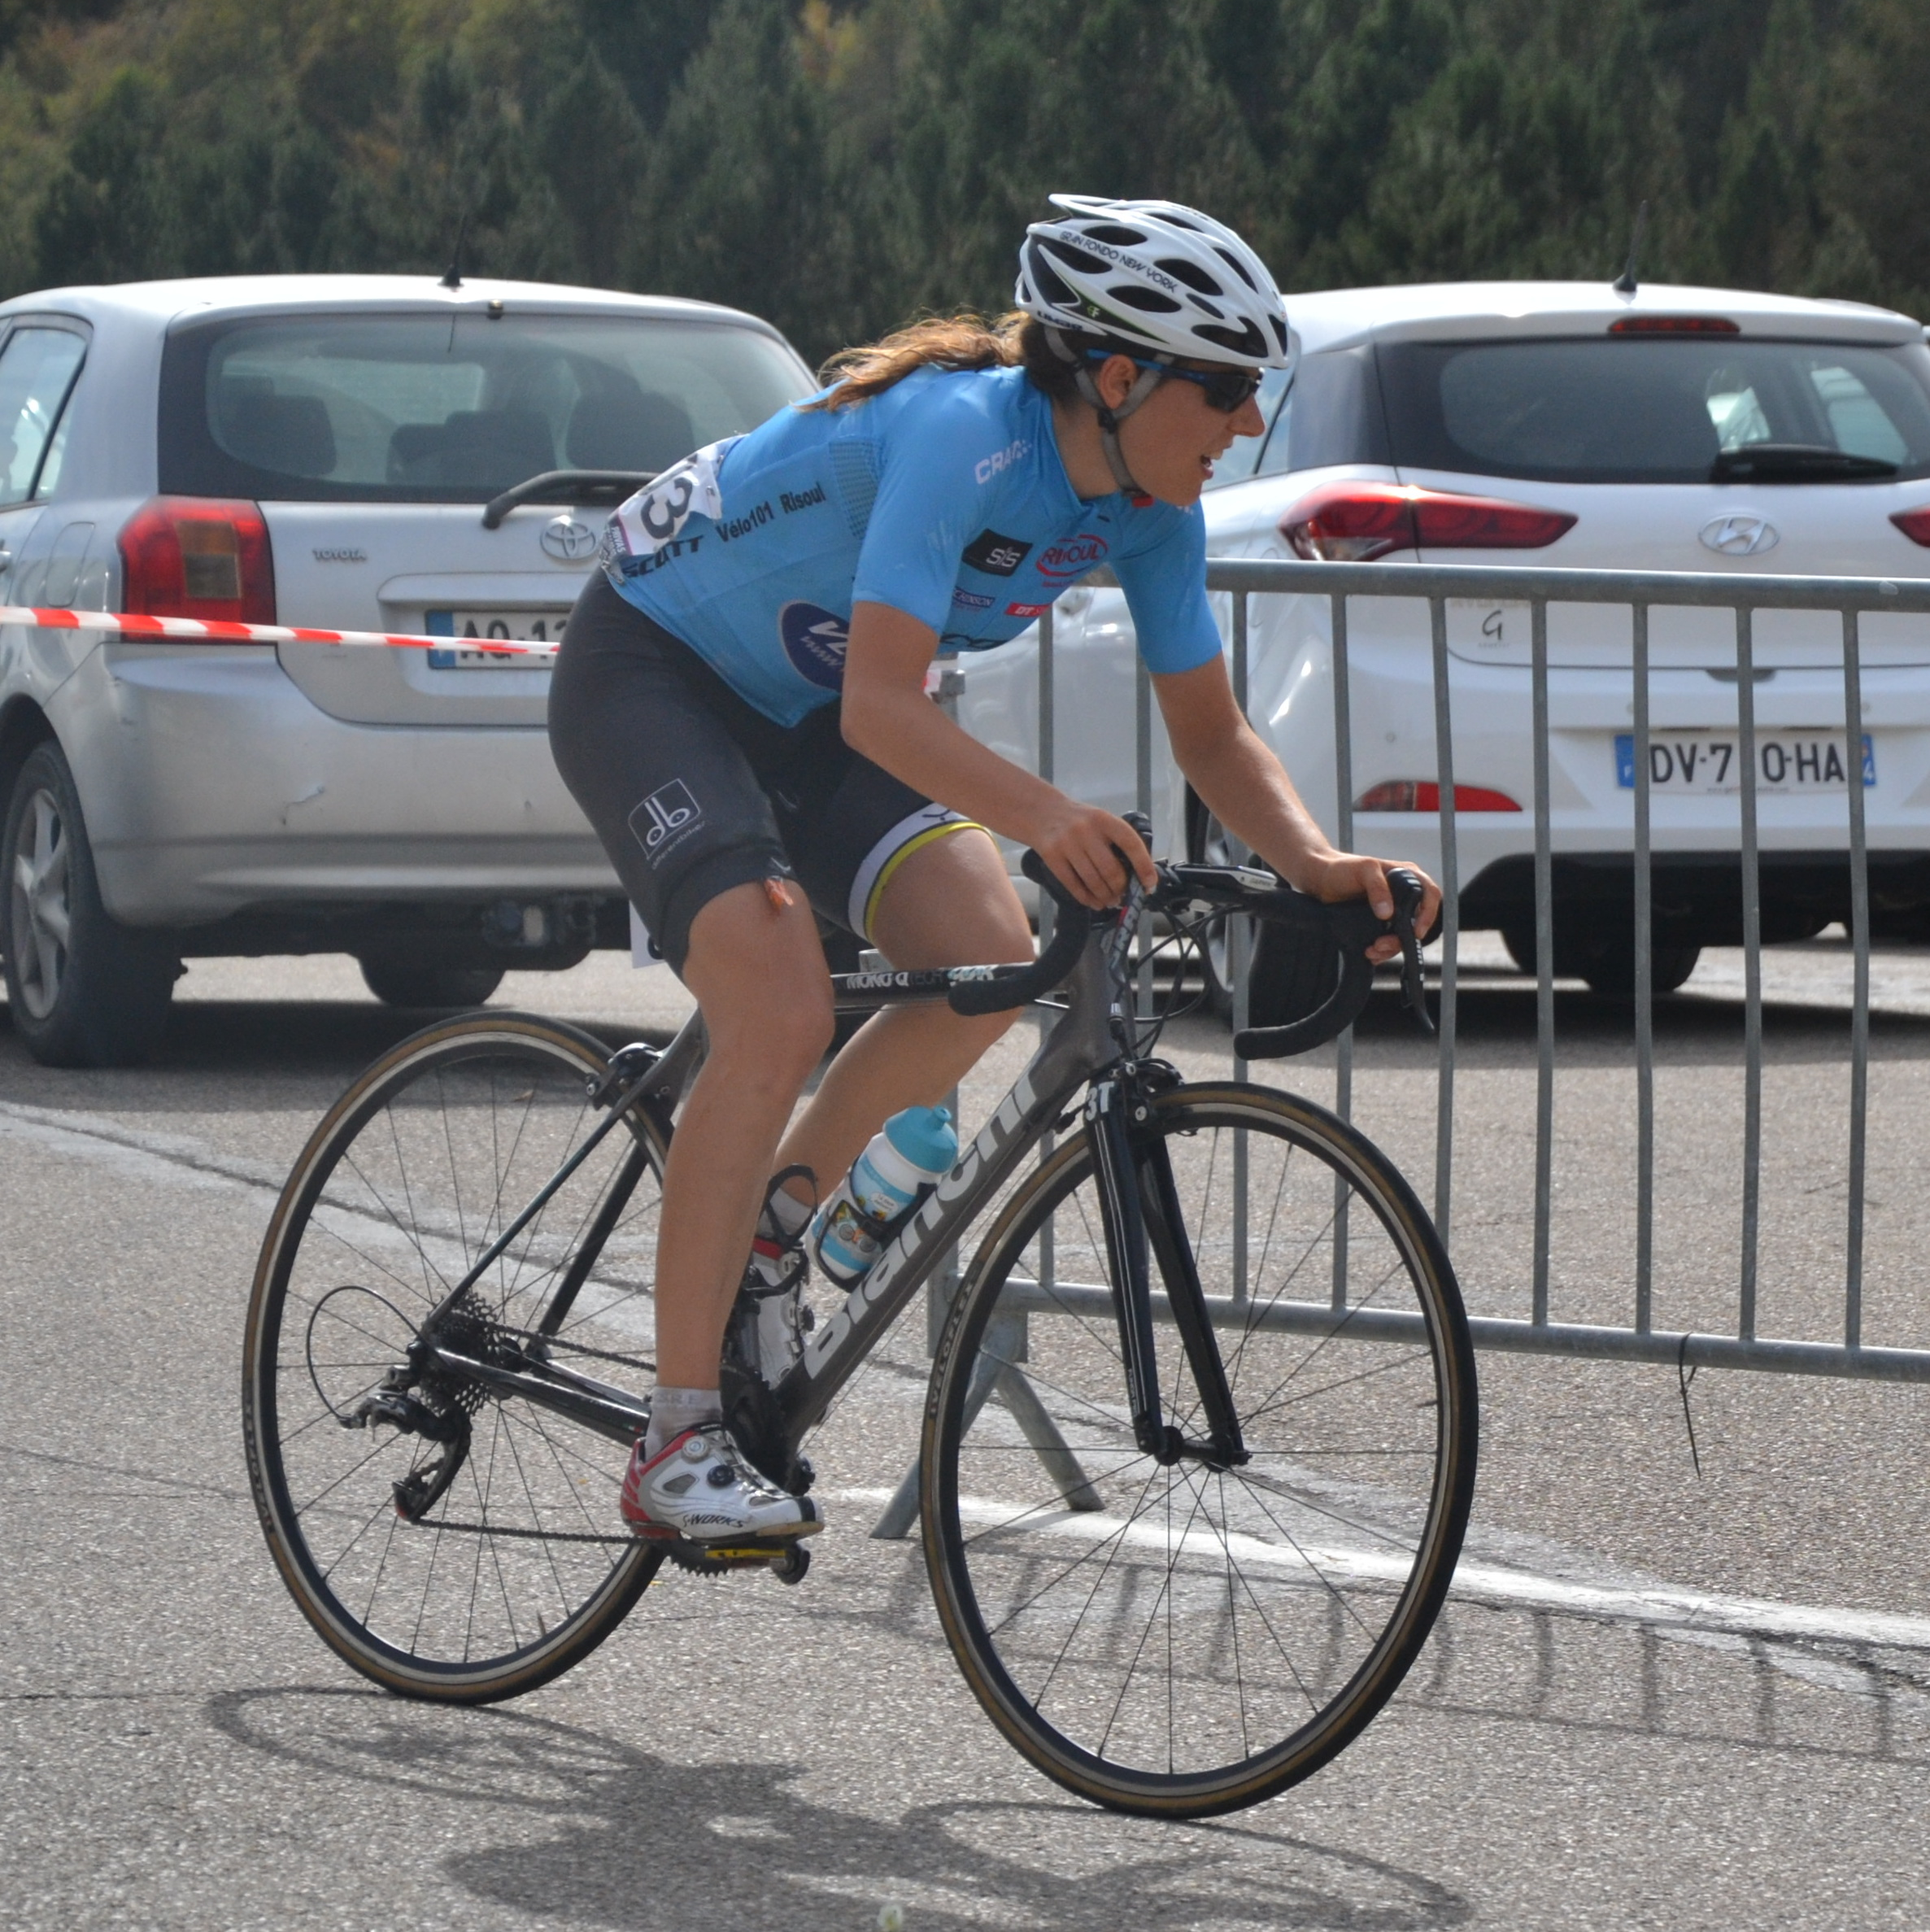
\includegraphics[width=0.9\textwidth]{fahrrad.jpg}
\end{center}
\end{column}


\end{columns}




\begin{itemize}
\item
Winkelgeschwindigkeit (Einheit: \(\frac{\text{rad}}{s}\)): Geschwindigkeit, mit der sich der Winkel verändert. 
\[
\omega = \frac{d\phi}{dt} 
\]
\\
\item
Bahngeschwindigkeit: Geschwindigkeit an der Außenseite des Rads (mit Radius \(r\)). 
\[
v = \omega \times r
\]
Einheit: \(\frac{m}{s}\)
\end{itemize}


\end{frame}




%% # Definition und Einheit von Winkelgeschwindig-
%% # keit und Winkelbeschleunigung,
%% # Mittelwert und Momentanwert

%% # gleichförmige Kreisbewegung,
%% # Zusammenhang zwischen Bahn- und Winkelge-
%% # schwindigkeit, Zentripetalbeschleunigung





\section{Kraft und Impuls}

\begin{frame}
\frametitle{Wie passiert Beschleunigung?}

Durch Einwirken von Kraft 

\begin{columns}[c]


\begin{column}{5cm}

\begin{center}
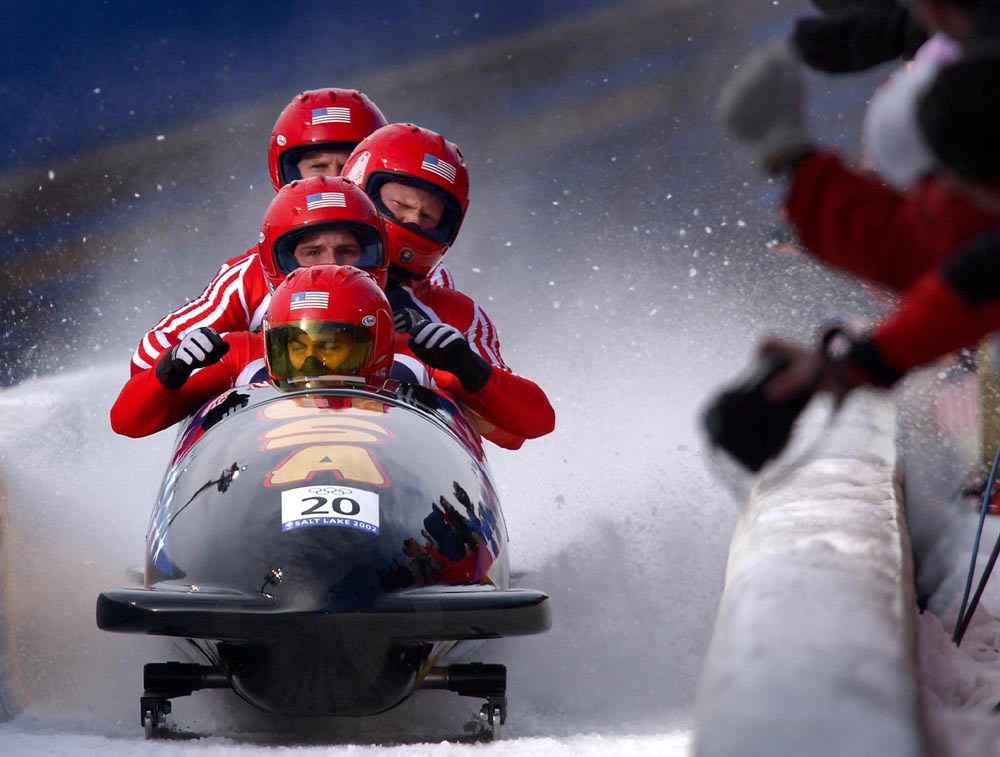
\includegraphics[width=\textwidth]{BobsledRun.jpg}
\end{center}


\end{column}

\begin{column}{6cm}


Kraft = Masse \(\times\) Beschleunigung 

\[F = m\times a\]

Einheit: \(kg\times\frac{m}{s^2} = \text{Newton (N)}\)


\end{column}

\end{columns}


\end{frame}

\begin{frame}
\frametitle{Beispiel: Freier Fall}


\begin{columns}[c]

\begin{column}{2cm}

\begin{center}
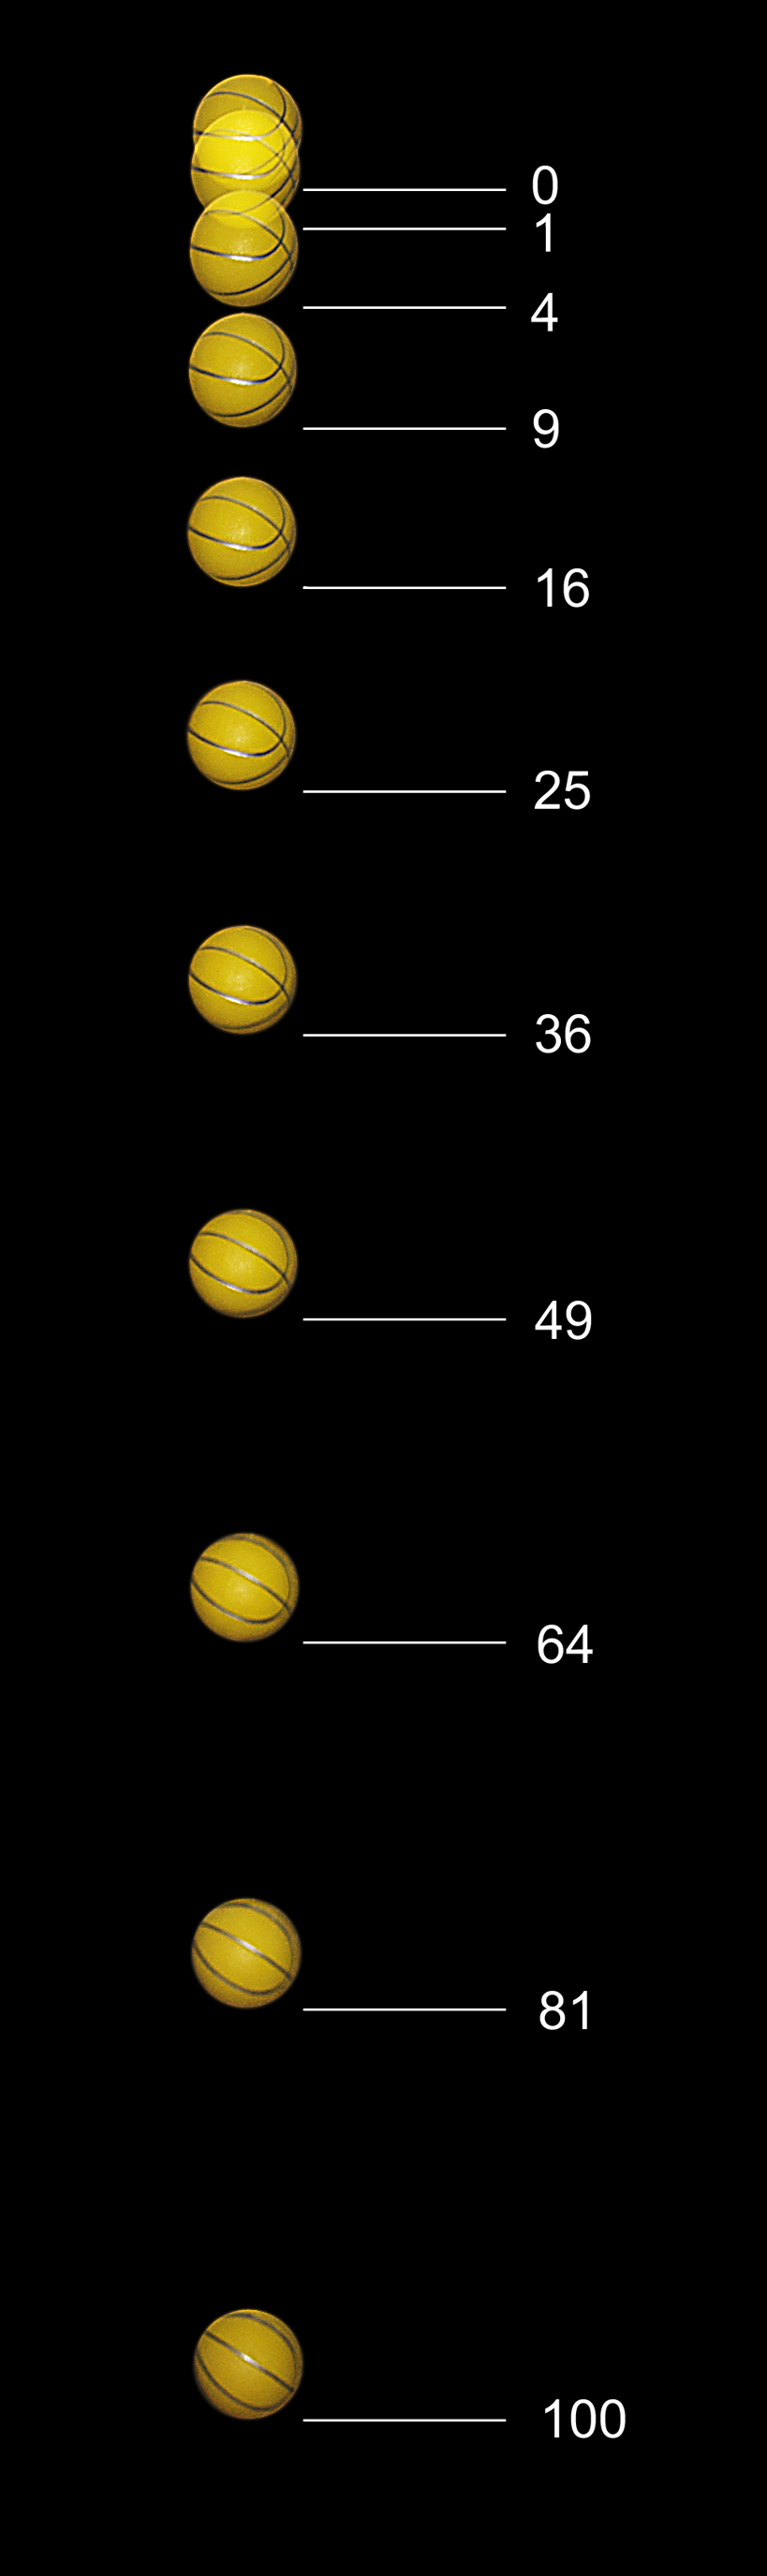
\includegraphics[width=0.9\textwidth]{freier_fall.jpg}
\end{center}


\end{column}



\begin{column}{8cm}
Fallende Objekte werden von der Schwerkraft beschleunigt. 

Die Beschleunigung ist hier die Fallbeschleunigung auf der Erde \(g \sim 10\,\frac{m}{s^2}\) \\[0.5 cm]

\pause

Beispiel: Basketball: \(\sim 600\,\text{g}\)

 
\pause

\[F = m\times a = 0.6\text{kg} \times 10 \frac{m}{s^2} \sim 6\,\text{N}\]

\end{column}





\end{columns}


\end{frame}



%% # Newtonsche Axiome,

\begin{frame}
\makebox[\linewidth]{\includegraphics[page=23,width=\textwidth]{Walter_Mechanik.pdf}}
\end{frame}





%% # Definition und Einheit von Impuls, Kraft und
%% # Kraftstoß,
%% # Impulserhaltungssatz,
%% # Gewichtskraft,
%% # Auftriebskraft (Schwimmen, Schweben, Sinken),
%% # Federkraft,
%% # Trägheitskräfte,
%% # Zentripetalkraft,
%% # Zentrifugalkraft,
%% # Reibungskraft zwischen festen Körpern:
%% # Haft-, Gleit- und Rollreibung, Reibungskoeffi-
%% # zienten, Schmiermittel

\begin{frame}
\frametitle{Impuls}

``Wucht'': Produkt aus Masse und Geschwindigkeit eines Körpers in Bewegung. Einheit: \(\
text{kg}\,\text{m}\,\text{s}^{-1}\)

\pause

Impulserhaltung: Der Gesamtimpuls eines geschlossenen Systems bleibt gleich* 

\begin{center}
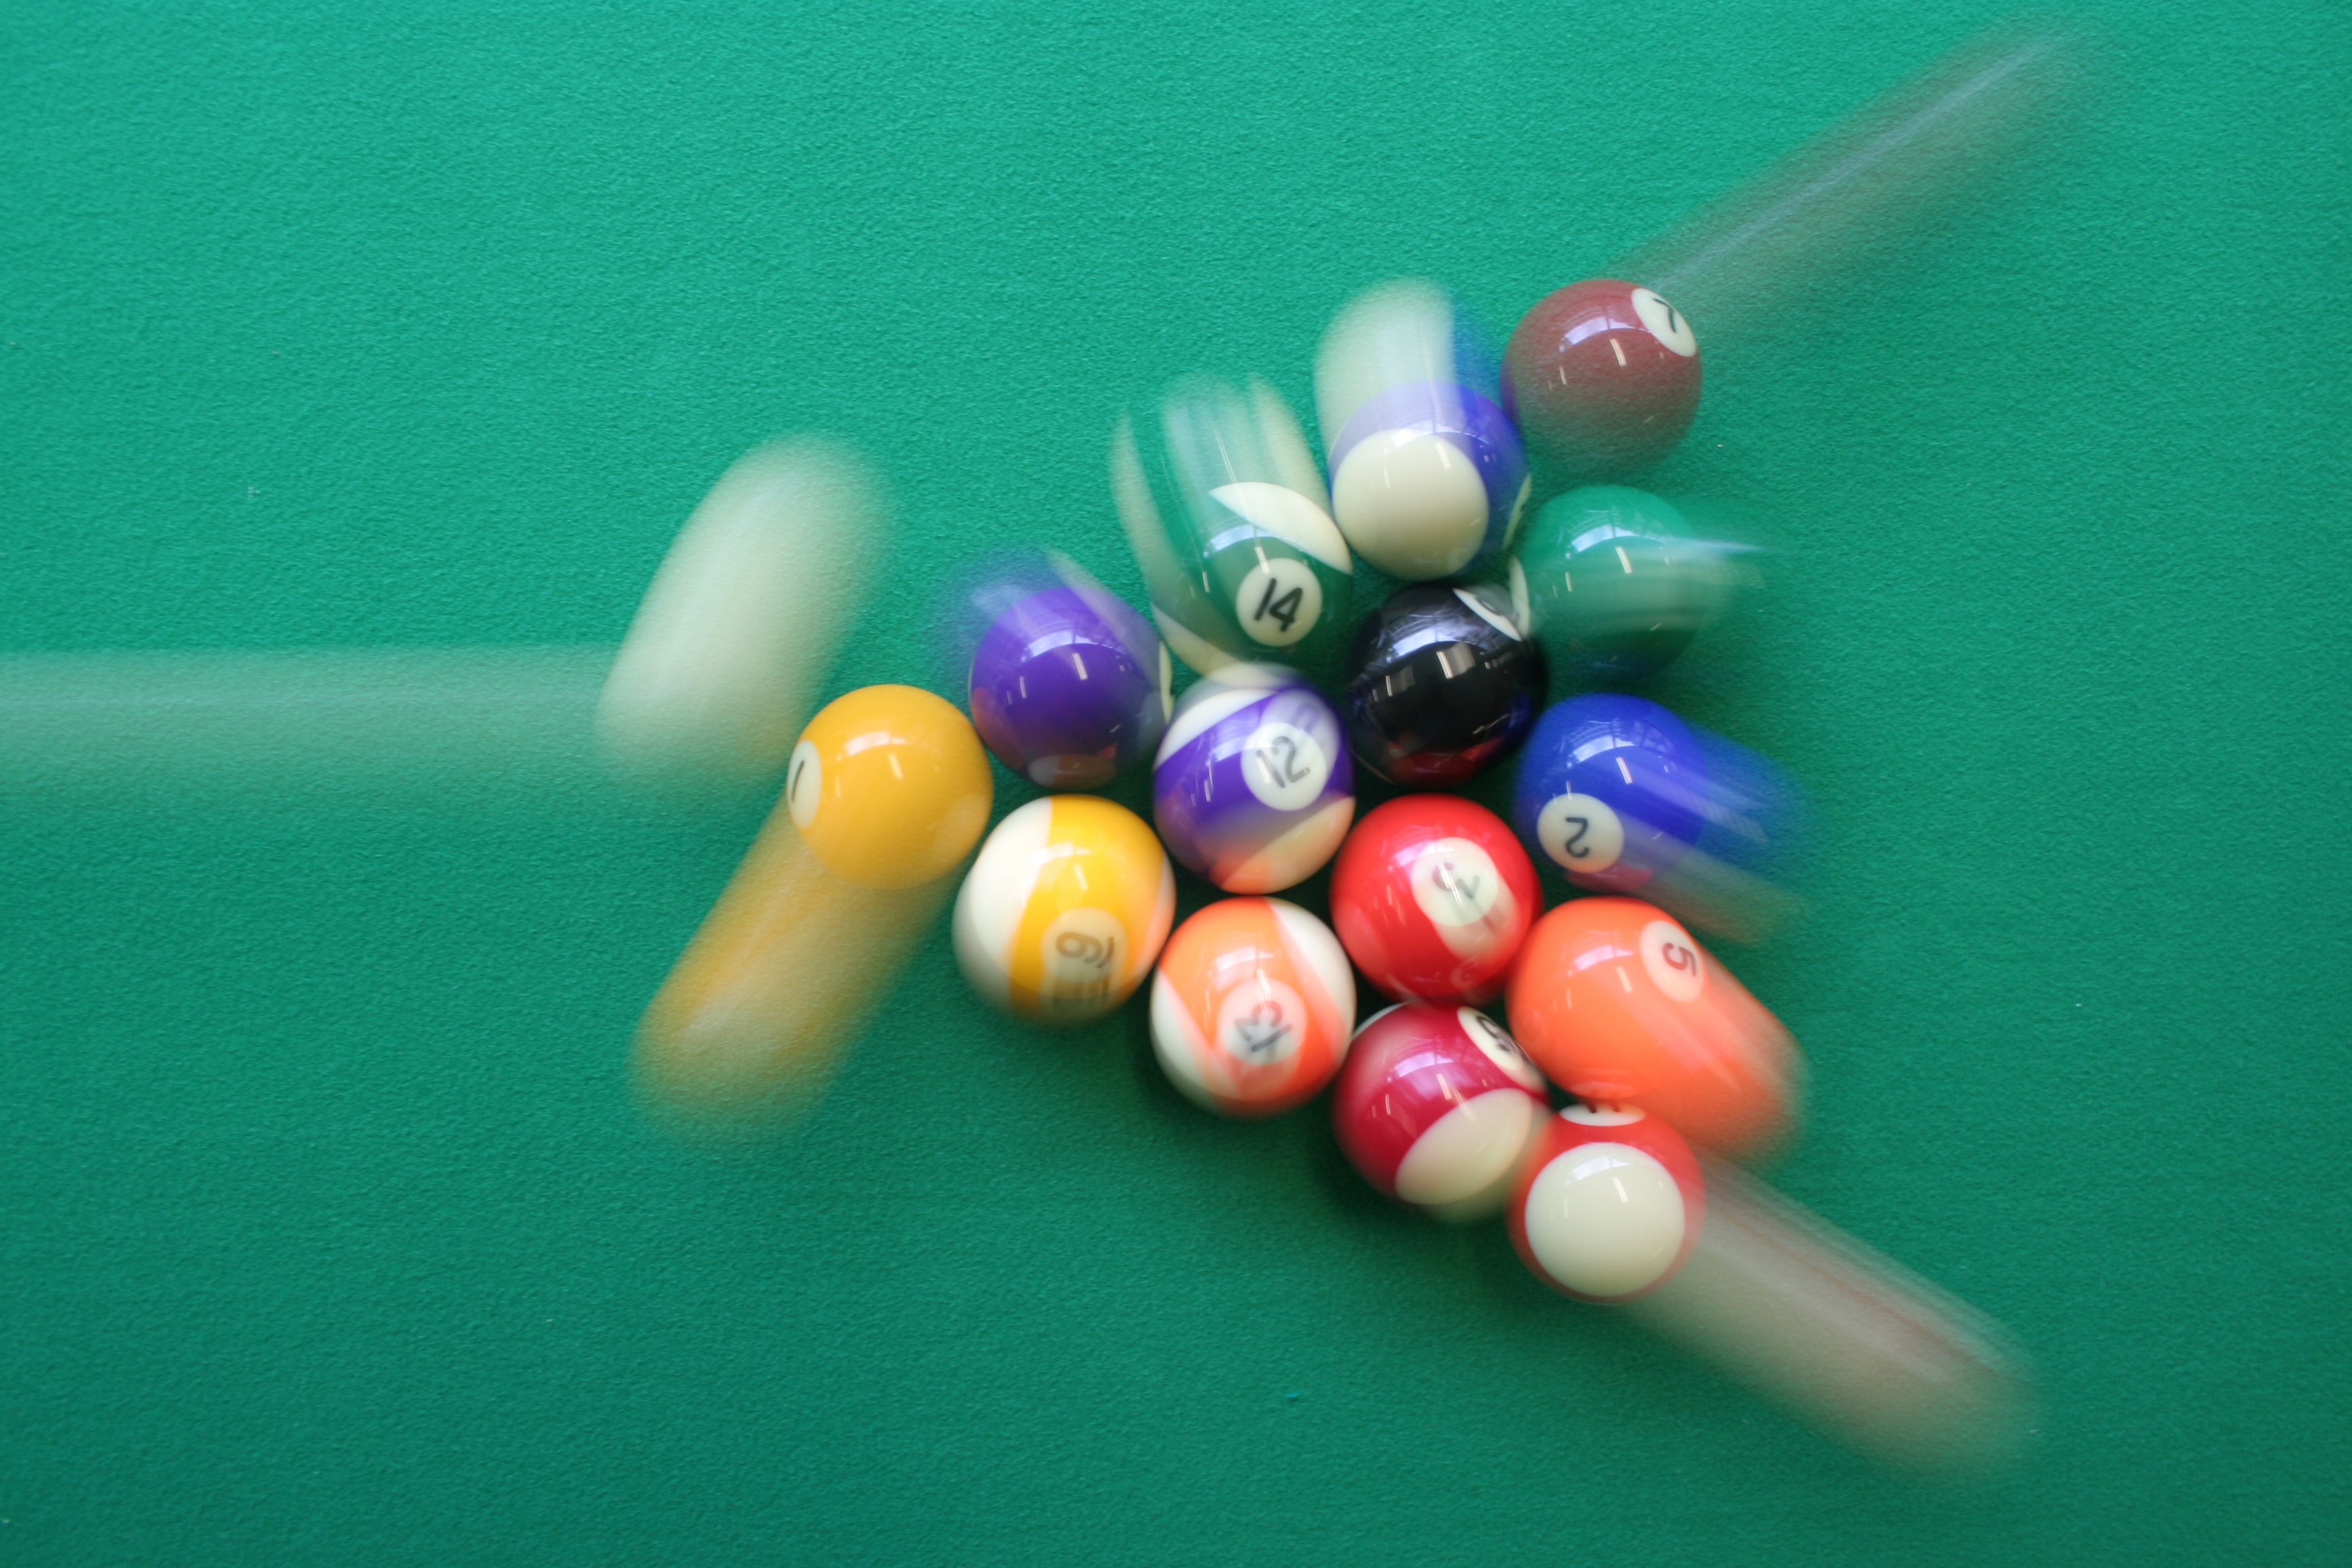
\includegraphics[width=0.3\textwidth]{billard.jpg}
\end{center}



 *Hier und bei allen anderen  Erhaltungssätzen: theoretisch (bis auf Reibungsverluste)
\end{frame}








% %% # Geschwindigkeitsproportionale Reibungskraft auf
% %% # einen in einer Flüssigkeit fallenden Körper,
% %% # Definition und Einheit der dynamischen Viskosität
% %% # (Koeffizient der inneren Reibung),
% %% # Sedimentationsgeschwindigkeit,
% %% # Viskosimeter,
% %% # Temperaturabhängigkeit der dynamischen Vis-
% %% # kosität


% %% # Sedimentation mit Hilfe einer Zentrifuge/Ultra-
% %% # zentrifuge,
% %% # Sedimentationskonstante (Verhältnis aus Sedi-
% %% # mentationsgeschwindigkeit und Zentrifugal-
% %% # beschleunigung)



\section{Arbeit, Energie, Leistung}


\begin{frame}
\frametitle{Arbeit}

Arbeit (W) ist das Produkt aus Kraft und Weg (in die Richtung, in die die Kraft geht):

\[W = F\times s\]

Einheit: Newton\(\times\)meter (Nm) = Joule (J)  

\end{frame}


\begin{frame}
\frametitle{Arbeit}


 
\begin{center}
\includegraphics<1>[width=0.7\textwidth]{serpentine.jpg}
%% \includegraphics<2>[width=0.7\textwidth]{serpentine_anno.png}
\end{center}

Die Arbeit, um von A nach B zu kommen, ist die gleiche, aber ein längerer Weg bedeutet weniger Kraft. 



\end{frame}

\begin{frame}
\frametitle{Aber warum ist die Arbeit um von A nach B zu kommen die gleiche?}

Weil es nur darum geht, den Energieunterschied zwischen A und B zu bewältigen. Energie = ``gespeicherte Arbeit'' (auch in Joule)

\pause

\begin{center}
%% 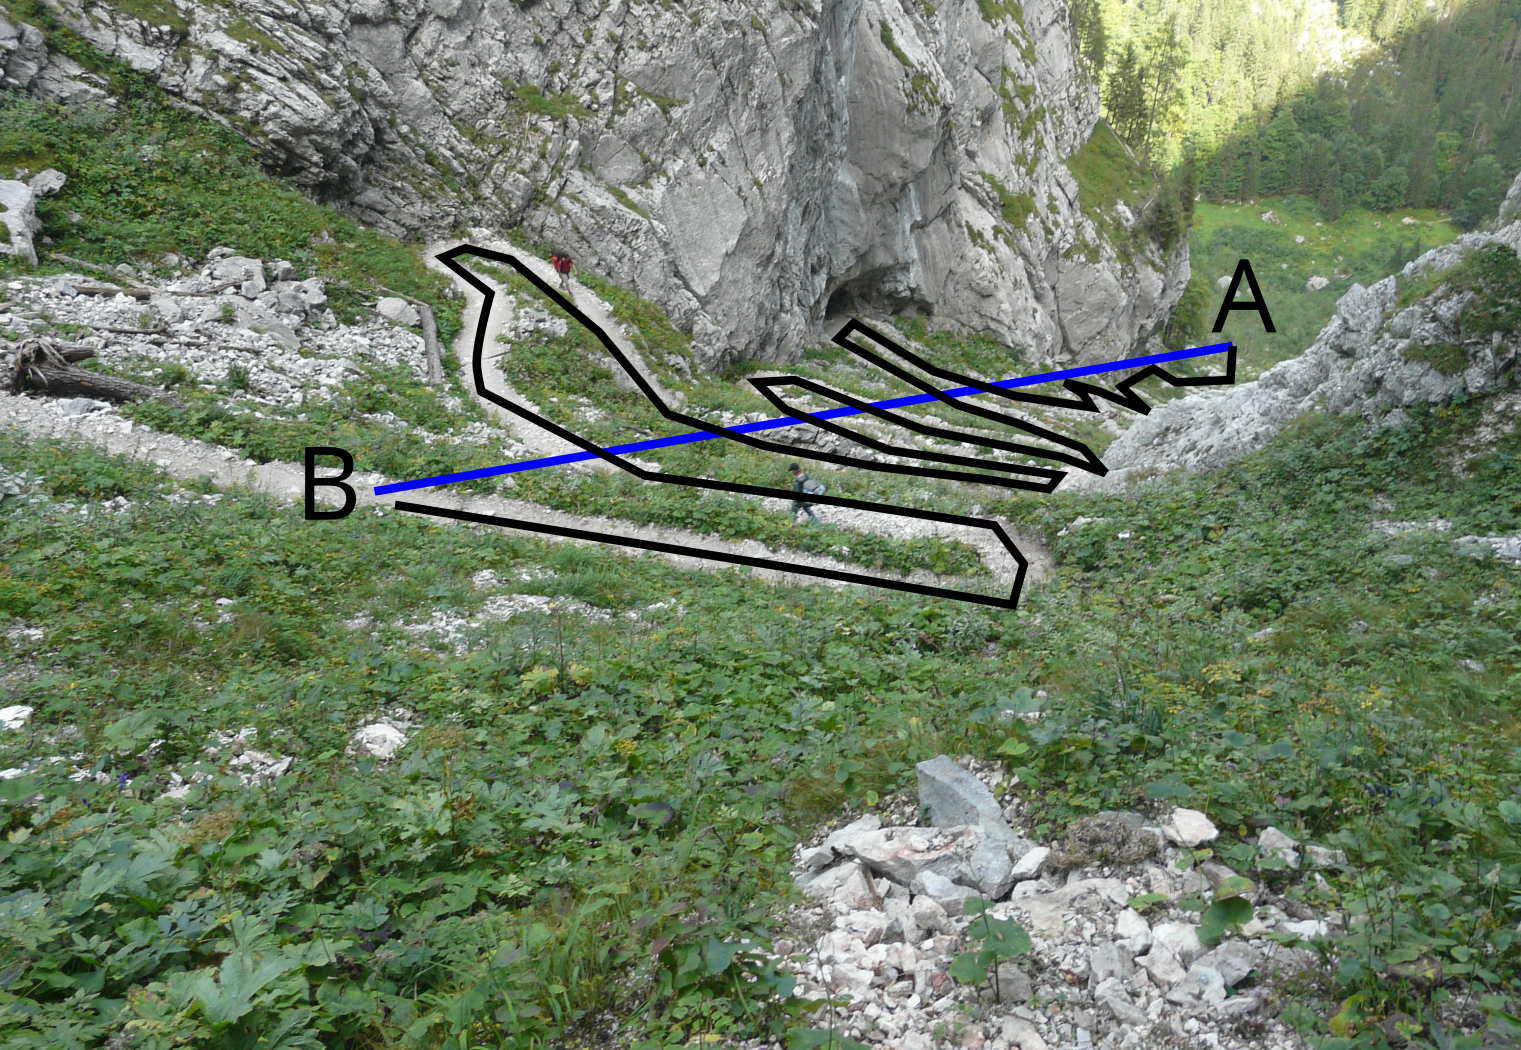
\includegraphics[width=0.7\textwidth]{/home/melanie/Work/pictures/physics/serpentine_anno.png}
\end{center}


\end{frame}


\begin{frame}
\frametitle{Arten von Energie}

\begin{itemize}
\item
Bewegungsenergie (kinetische Energie)
\item
Lageenergie (potentielle Energie)
\item
Verformungsenergie
\item
thermische Energie
\item
chemische Energie
\item
elektrische Energie
\end{itemize}

\end{frame}


\begin{frame}
\frametitle{Energieerhaltung}

\begin{columns}[c]

\begin{column}{5cm}
Arten von Energie können ineinander umgewandelt werden, aber die Gesamtenergie in einem geschlossenen System ist konstant. \\

\pause

Beispiel: Stabhochsprung

\end{column}

\begin{column}{5cm}
\begin{center}
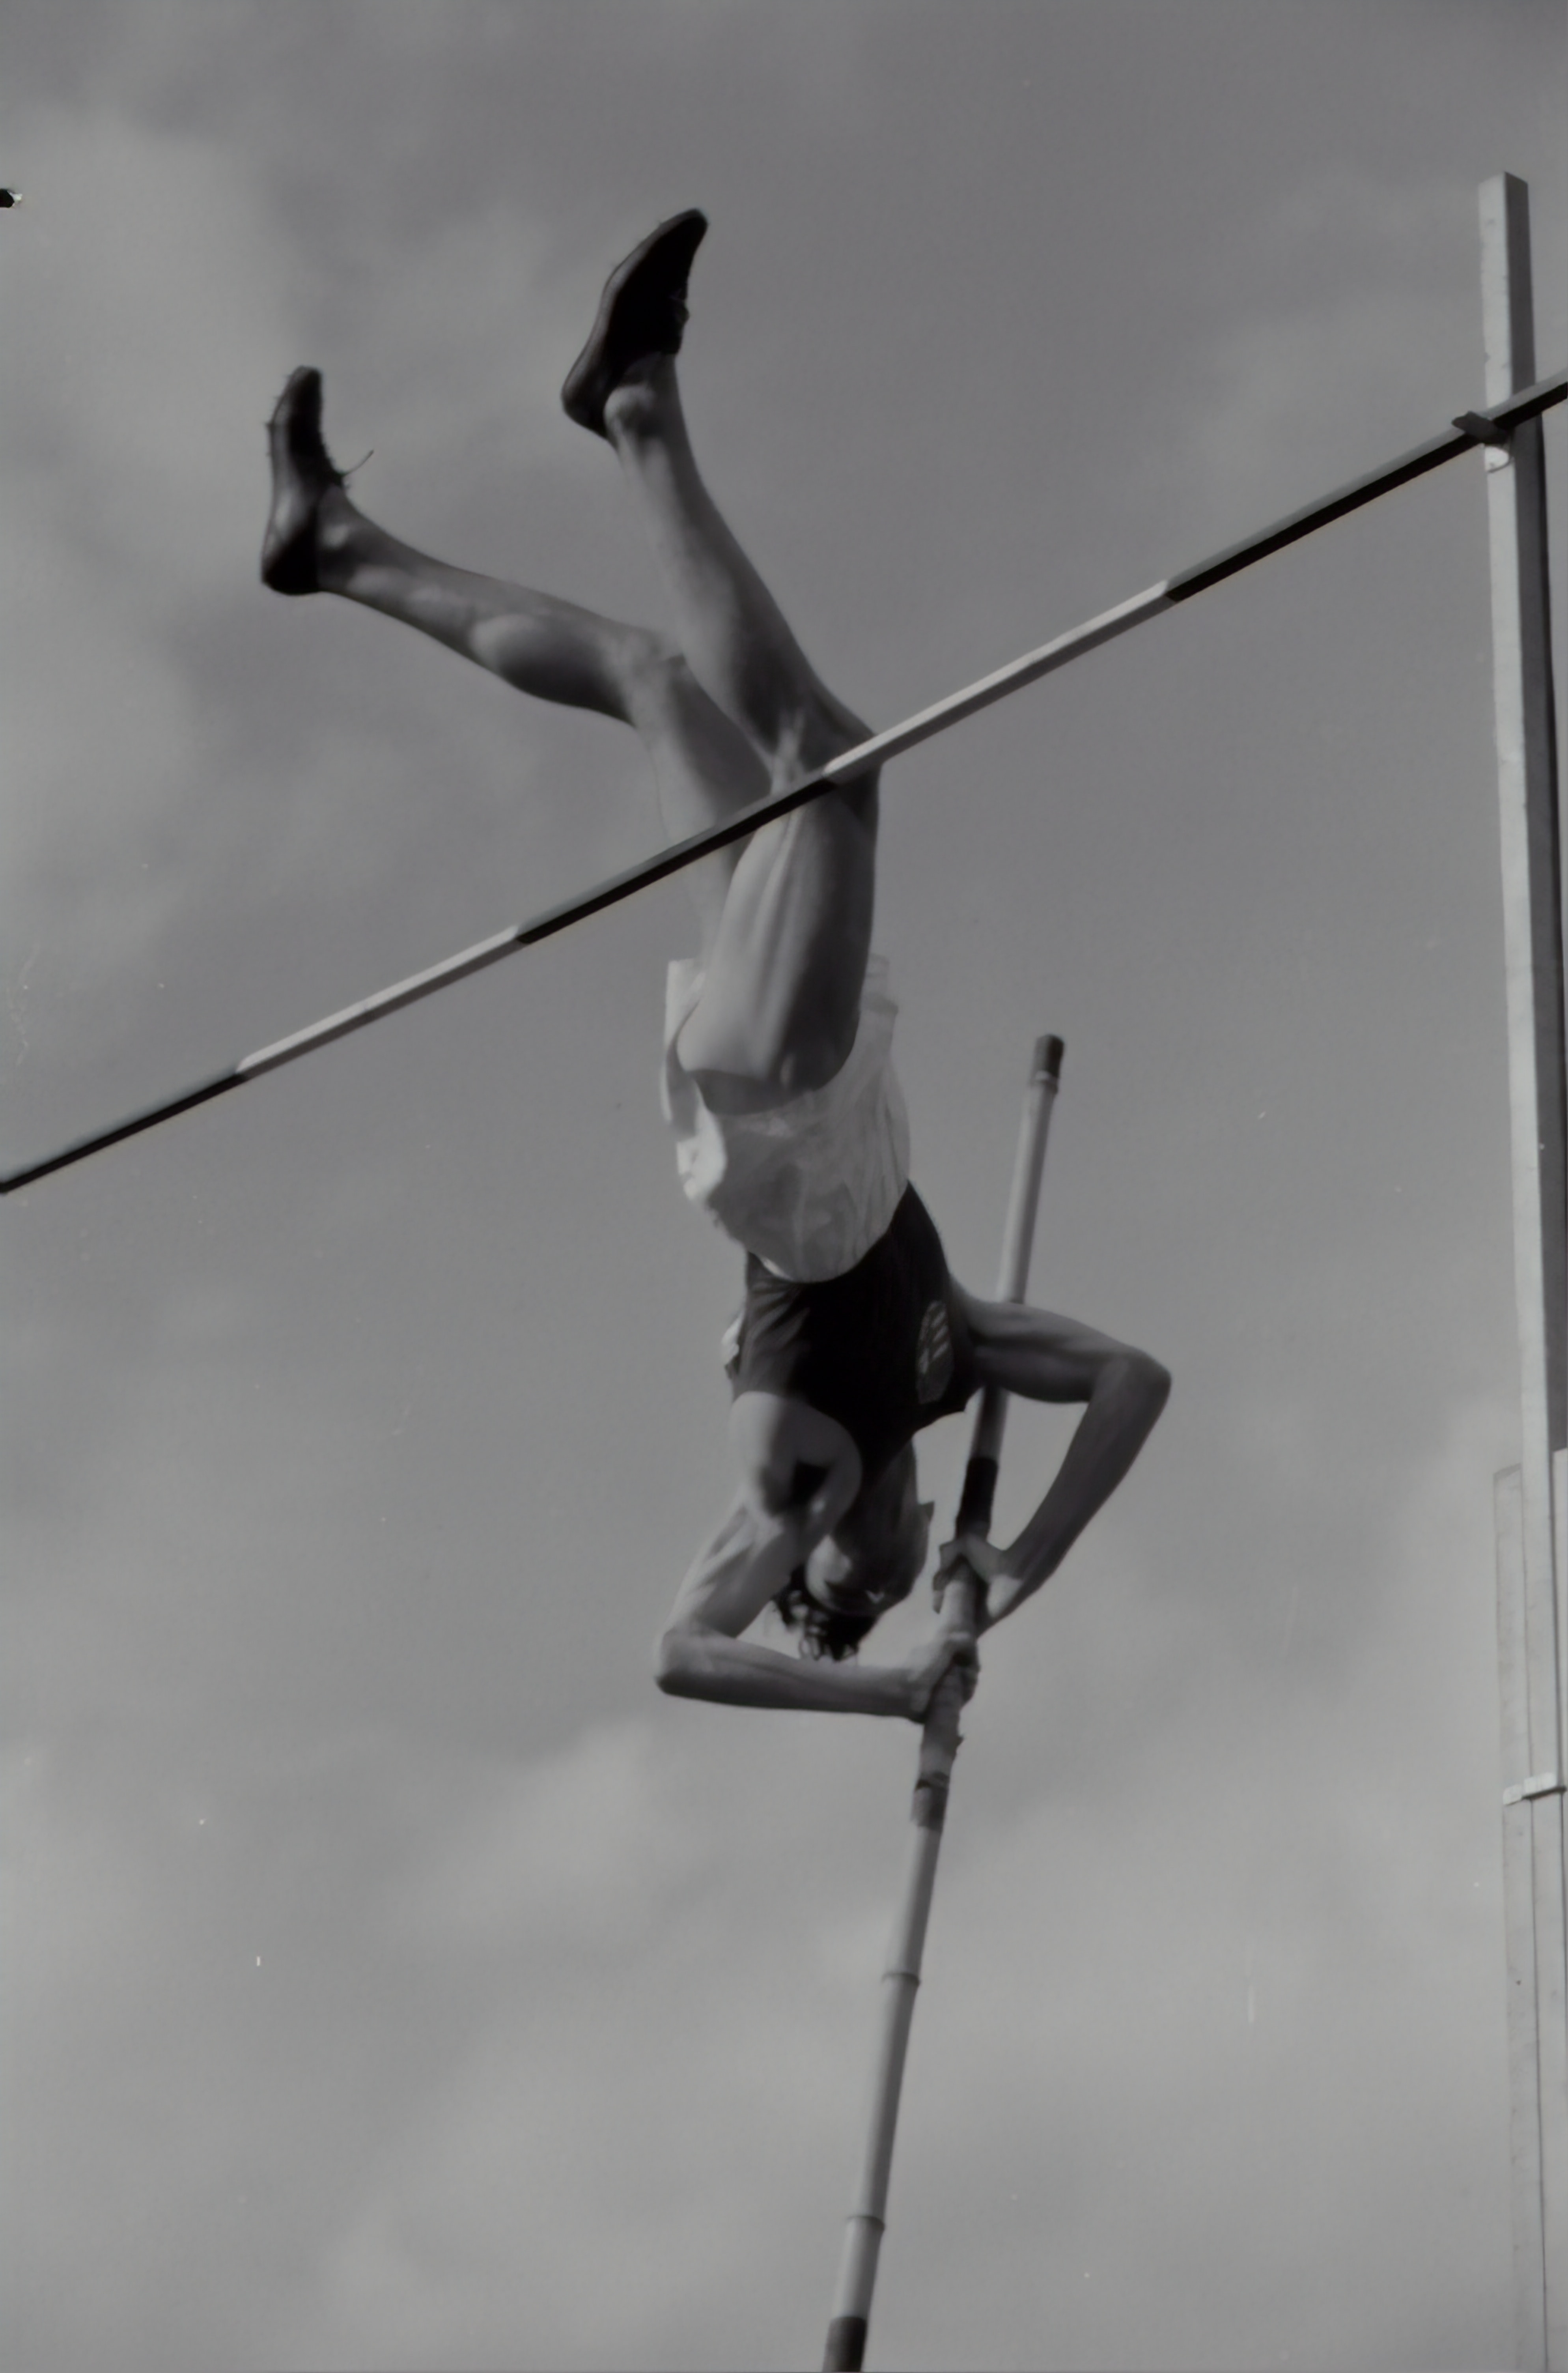
\includegraphics[width=0.9\textwidth]{stabhochsprung.jpg}
\end{center}
\end{column}

\end{columns}

\end{frame}


%% # Definition und Einheit der Leistung,

\begin{frame}
\frametitle{Zurück zur Arbeit}

 
\begin{columns}[c]

\begin{column}{5cm}

\begin{center}
%% 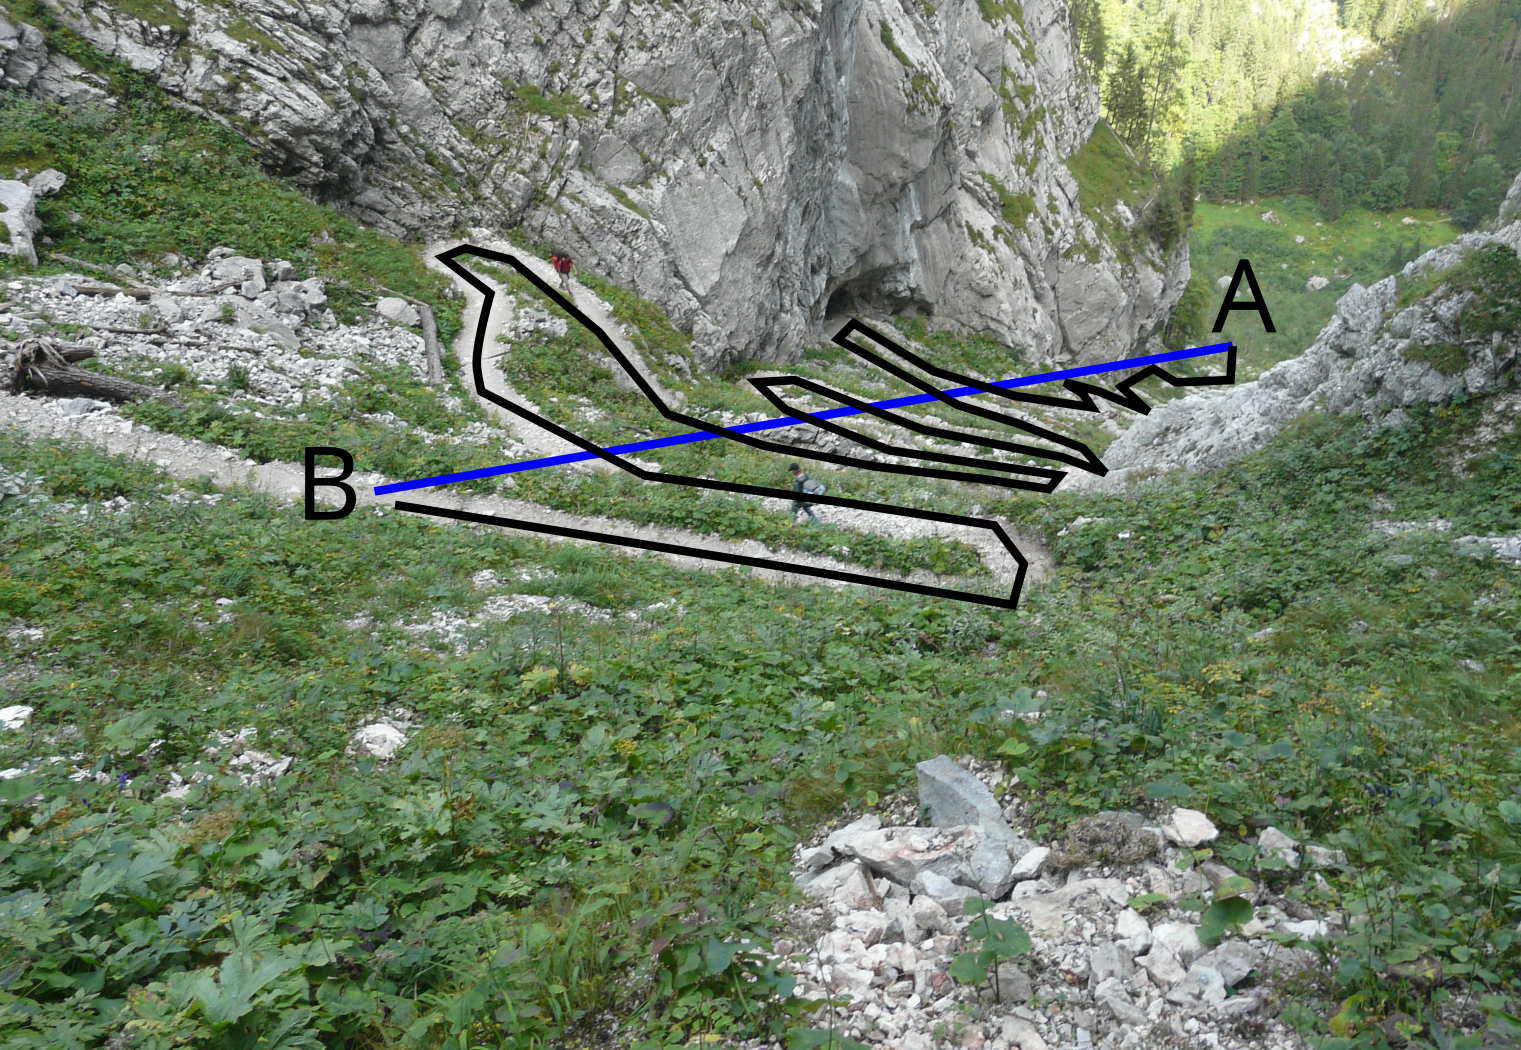
\includegraphics[width=\textwidth]{/home/melanie/Work/pictures/physics/serpentine_anno.png}
\end{center}

\end{column}

\begin{column}{5cm}


Ist es eigenartig, dass die Arbeit auf beiden Wegen die gleiche ist? \pause

Die \emph{Arbeit} ist gleich, aber die \emph{Leistung} ist unterschiedlich! 

\[
\text{Leistung} = \frac{\text{Arbeit}}{\text{Zeit}}
\]

Einheit: Watt (W): \(1\,W = 1\,\frac{J}{s}\)
\end{column}



\end{columns}

\end{frame}


\section{Drehmoment, Trägheitsmoment, Drehimpuls}

%% # Definition und Einheit von Drehmoment,
%% # Hebelgesetz


\begin{frame}
\makebox[\linewidth]{\includegraphics[page=39,width=\textwidth]{Walter_Mechanik.pdf}}
\end{frame}

\begin{frame}
\makebox[\linewidth]{\includegraphics[page=40,width=\textwidth]{Walter_Mechanik.pdf}}
\end{frame}
 
%% Beispiel: Rudern
\begin{frame}
\frametitle{Beispiel}

\begin{center}
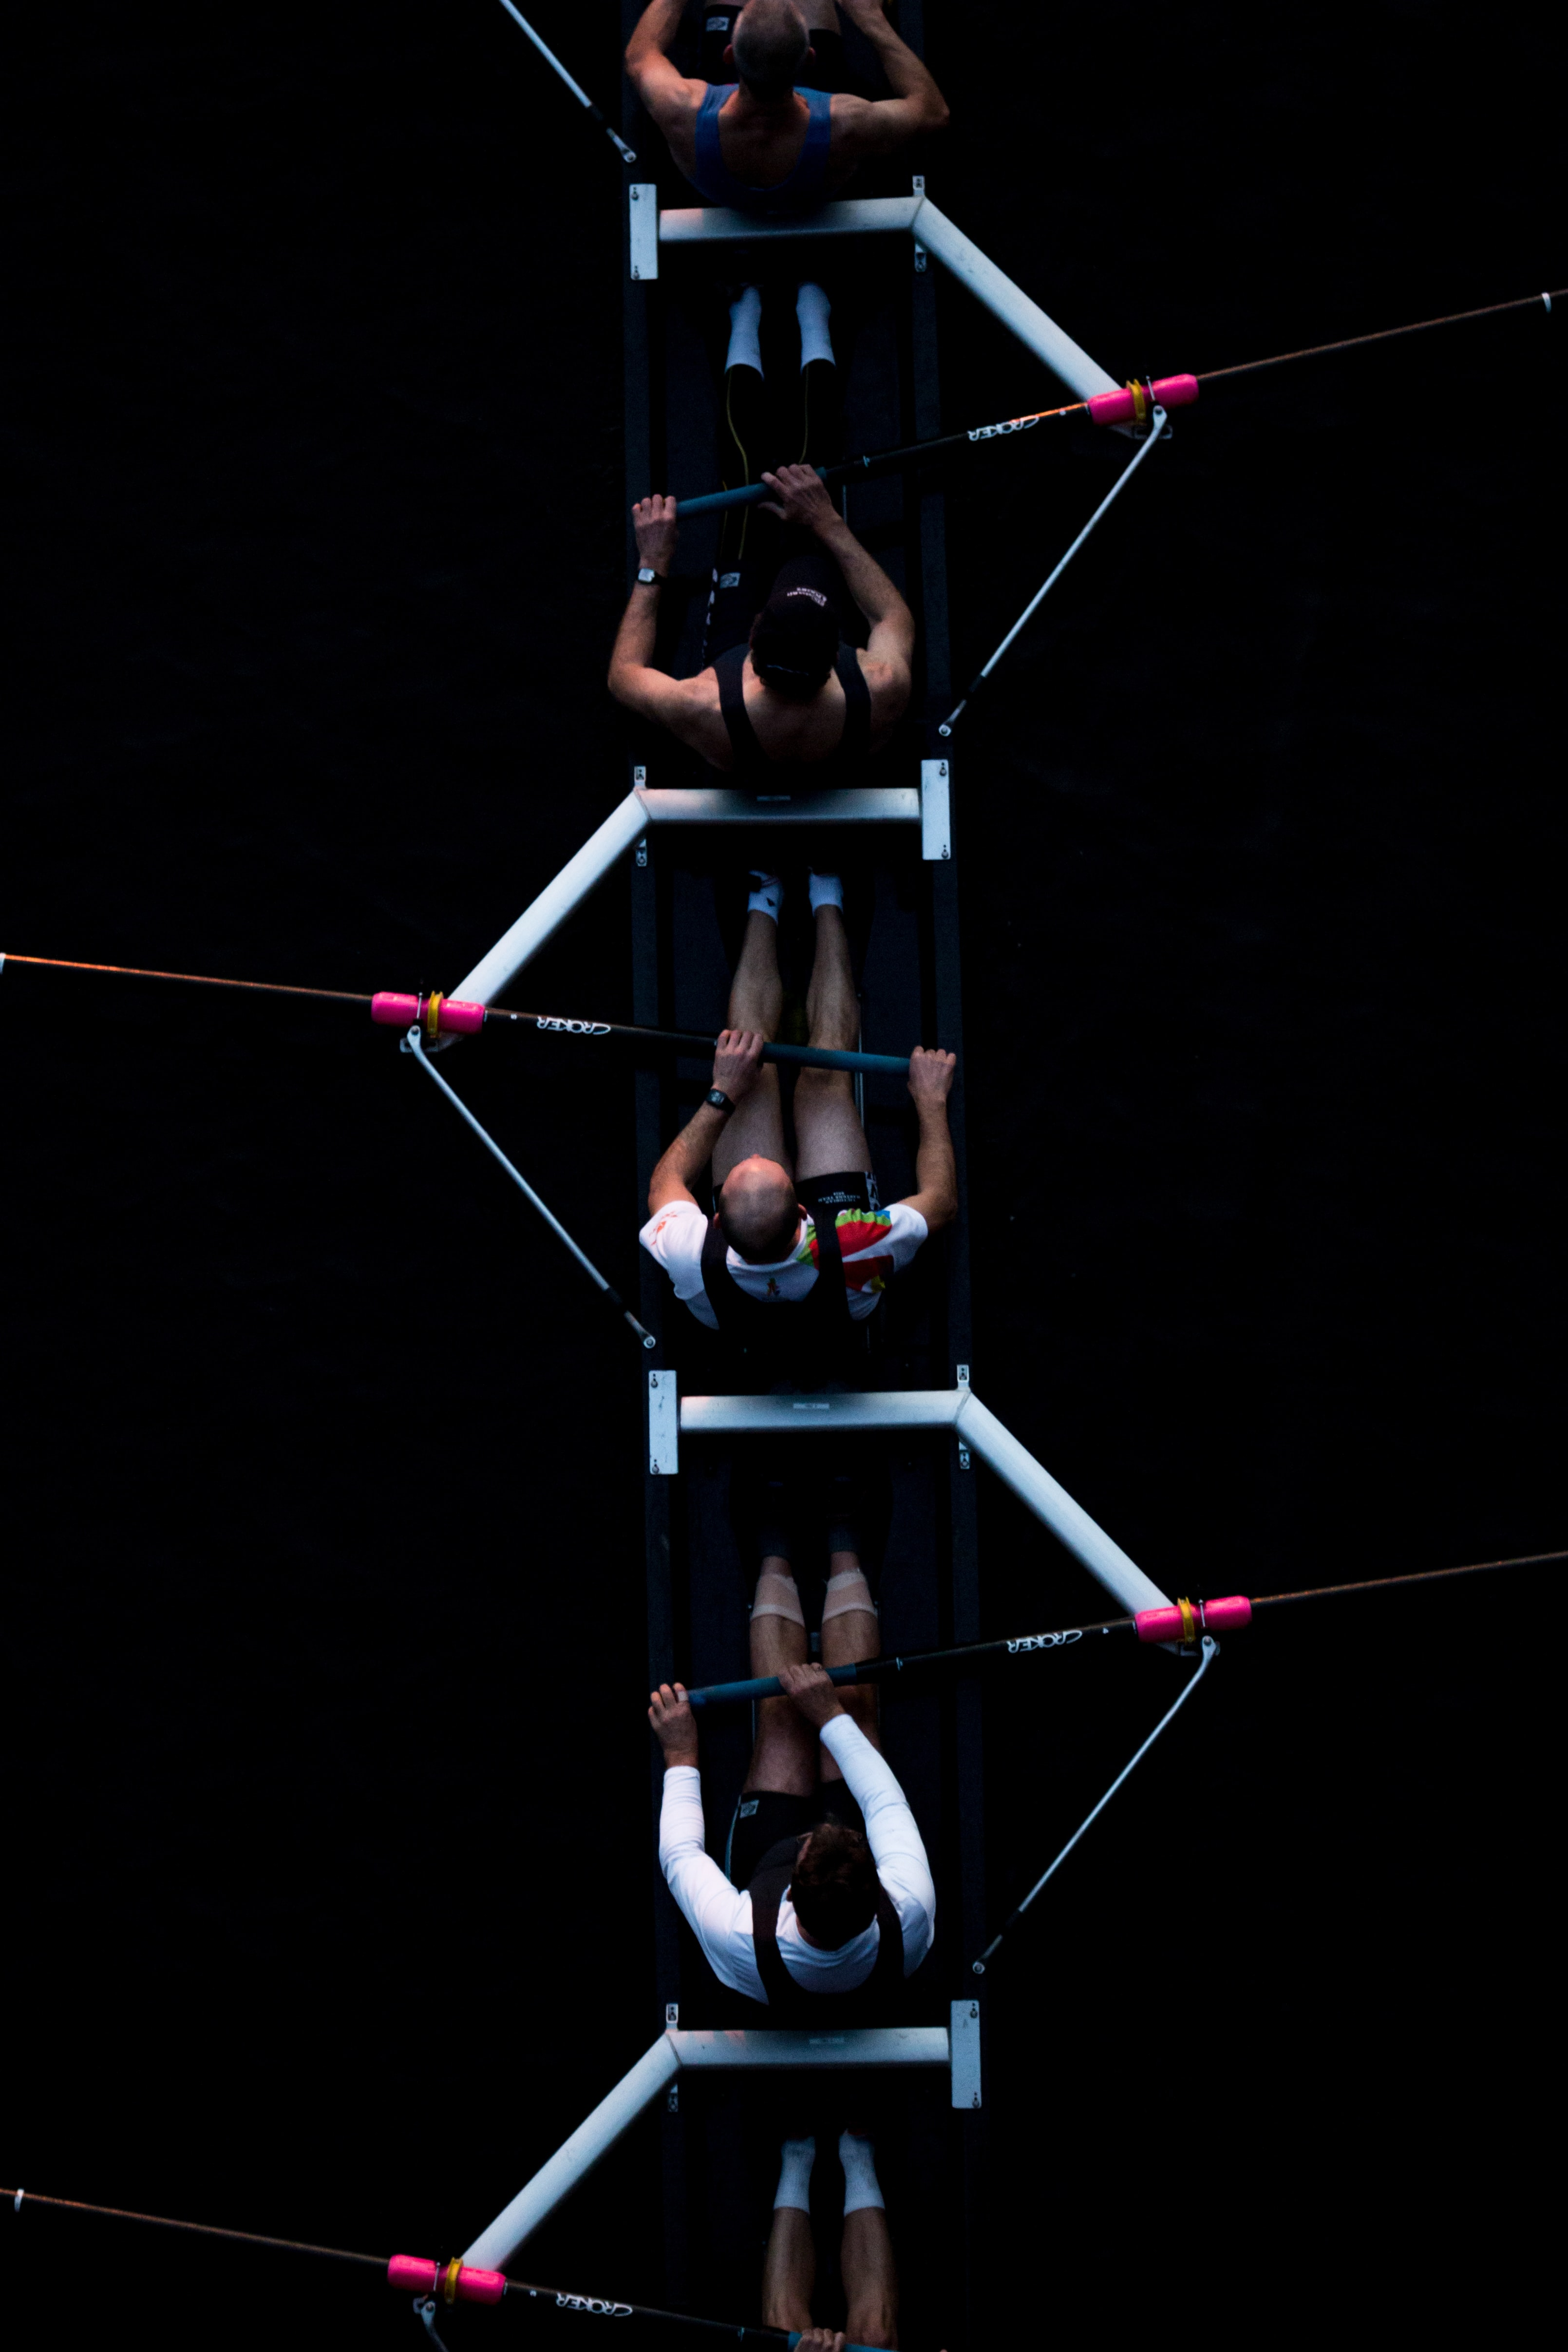
\includegraphics[width=0.9\textwidth]{rowing.jpg}
\end{center}

\end{frame}
 






%% # Definition und Einheit von Trägheitsmoment
%% # und Drehimpuls,
%% # Drehimpulserhaltung

\begin{frame}
\frametitle{Trägheitsmoment und Drehimpuls}


Trägheitsmoment I (Einheit:  kg\(\,\)m$^2$): Trägheit eines Körpers gegenüber Veränderungen in der Winkelgeschwindigkeit bei einer Drehbewegung. 

I ist größer, je mehr Masse weiter von der Drehachse entfernt ist. 




\end{frame}


\begin{frame}
\frametitle{Drehimpuls}

Drehimpuls: Trägheitsmoment \(\times\) Winkelgeschwindigkeit \\ (Einheit: kg\(\,\)m$^2\,$s$^{-1}$)



\begin{columns}[c]

\begin{column}{5cm}



\[
L = I\times \omega
\]


Der Drehimpuls ist eine Erhaltungsgröße \\[0.2 cm]


Wie kann die Eisläuferin ihre Pirouette beschleunigen oder verlangsamen?


\end{column}

\begin{column}{5cm}


\begin{center}
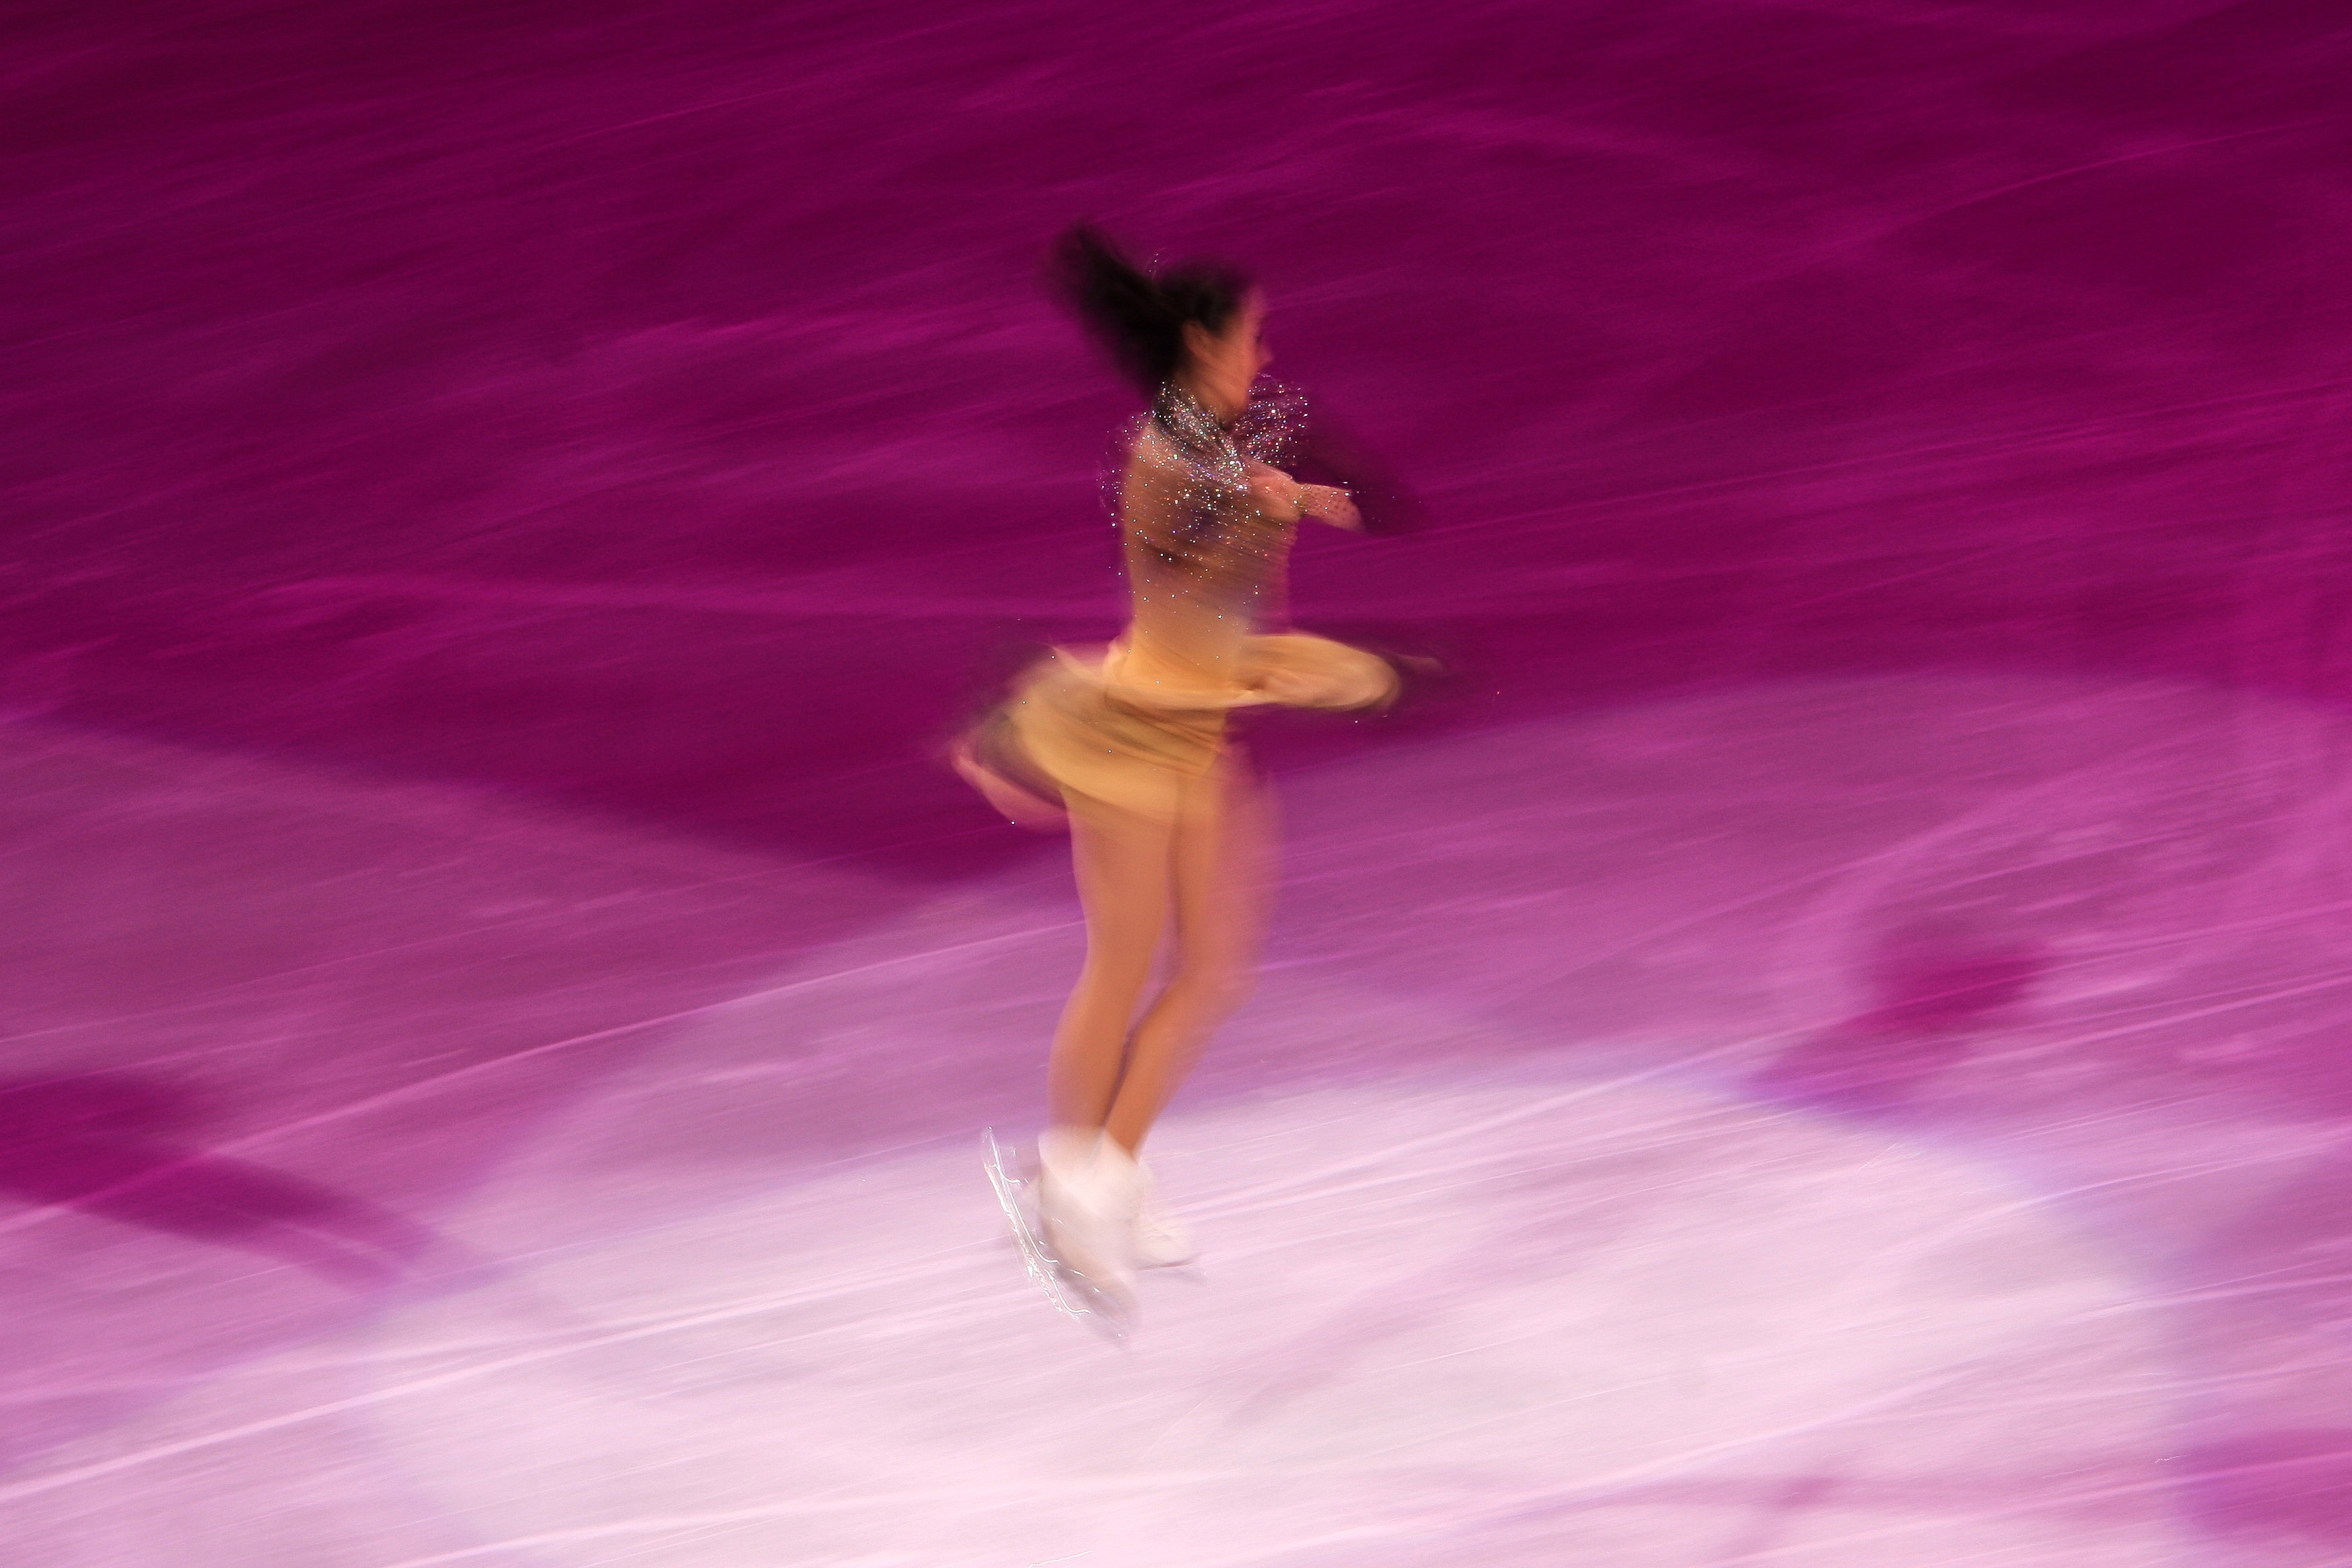
\includegraphics[width=0.9\textwidth]{figureskater.jpg}
\end{center}

\end{column}


\end{columns}


\end{frame}


%% Review

\begin{frame}

\frametitle{Jetzt* sollten Sie:}



\begin{block}{Wissen:}
\begin{itemize}
\item
Zusammenhang zwischen Strecke, Geschwindigkeit und Beschleunigung erklären
\item
Periodendauer, Frequenz und Kreisfrequenz definieren
\item
die Newtonschen Axiome nennen
\item
Impuls und Kraft definieren
\item
den  Impulserhaltungssatz wiedergeben und Beispiele geben
\item
Arbeit, Leistung und Energie definieren
\item
Arten von Energie unterscheiden
\item
den Energieerhaltungssatz erklären
\item
Drehmoment definieren und das Hebelgesetz
\item
Trägheitsmoment und Drehimpuls definieren
\item
den Drehimpulserhaltungssatz erklären und Beispiele nennen 
\end{itemize}

\end{block}

\end{frame}

\begin{frame}

\frametitle{Jetzt* sollten Sie:}
 



\begin{block}{Können:}
\begin{itemize}
\item
Bewegungsdiagramme lesen und verstehen/auswerten
\item
Mittelwert und Momentanwert der Geschwindigkeit errechnen
\item
Parameter einer Kreisbewegung berechnen
\item 
das Hebelgesetz anwenden
\end{itemize}
\end{block}


 
\begin{block}{Fühlen:}
\begin{itemize}
\item
mechanische Prozesse im täglichen Leben erkennen
\item
über Anwendungen von Mechanik in der Medizin nachdenken
\end{itemize}
\end{block}

 \end{frame}






\begin{frame}
\frametitle{Danke für Ihr Feedback!}

\begin{columns}[c]

\begin{column}{6cm}
\begin{center}
% 
\includegraphics[width=\textwidth]{/home/melanie/Work/pictures/metaphore/smilie_balloons.jpg}
\end{center}

\end{column}

\begin{column}{4cm}


\begin{center}
% 
\includegraphics[width=\textwidth]{feedback_QR.png}
\end{center}
\end{column}


\end{columns}

\end{frame}





%% Bildnachweis
\begin{frame}
\frametitle{Bildnachweis}
 
Diese Vorlesung verwendet teilweise Materialien (Folien und Bilder) einer früheren Vorlesung von Prof. Wim Walter.  

\vfill

\begin{tiny}
 
\begin{itemize}

\item
Anna Kiesenhofer auf einem Fahrrad. Von Marianne Casamance - Eigenes Werk, CC BY-SA 4.0, \url{https://commons.wikimedia.org/w/index.php?curid=51096042}

\item
Billardspiel. Von No-w-ay in collaboration with H. Caps - Eigenes Werk, CC BY-SA 4.0, \url{https://commons.wikimedia.org/w/index.php?curid=3216565}

\item
Freier Fall. Von MichaelMaggs - Eigenes Werk, CC BY-SA 3.0, \url{https://commons.wikimedia.org/w/index.php?curid=2946486}

\item
Logo der MSB. MSB Medical School Berlin, Public Domain, via Wikimedia Commons

\item
Luftballons mit frohen und traurigen Smileys. Photo by \href{https://unsplash.com/@artbyhybrid?utm_source=unsplash&utm_medium=referral&utm_content=creditCopyText}{Hybrid} on \href{https://unsplash.com/s/photos/feedback?utm_source=unsplash&utm_medium=referral&utm_content=creditCopyText}{Unsplash}
  
\item
Pirouette. Photo by \href{https://unsplash.com/@rodlong?utm_source=unsplash&utm_medium=referral&utm_content=creditCopyText}{Rod Long} on \href{https://unsplash.com/s/photos/figure-skater?utm_source=unsplash&utm_medium=referral&utm_content=creditCopyText}{Unsplash}  

\item
Ruderboot von oben. Photo by \href{https://unsplash.com/@joshcala?utm_source=unsplash&utm_medium=referral&utm_content=creditCopyText}{Josh Calabrese} on \href{https://unsplash.com/s/photos/rowing?utm_source=unsplash&utm_medium=referral&utm_content=creditCopyText}{Unsplash}
  

\item
Screenshot eines Artikels auf olympics.com, über Surferin Carissa Moore. \href{https://olympics.com/de/video/carissa-moore-air-surf-gravity-tokyo-finals}{https://olympics.com/de/video/carissa-moore-air-surf-gravity-tokyo-finals}, aufgerufen im April 2022.

\item
Stabhochsprung. Photo by \href{https://unsplash.com/@austriannationallibrary?utm_source=unsplash&utm_medium=referral&utm_content=creditCopyText}{Austrian National Library} on \href{https://unsplash.com/s/photos/pole-vault?utm_source=unsplash&utm_medium=referral&utm_content=creditCopyText}{Unsplash}

\item
Viererbob. Von 1st Class Preston Keres - US-Army images, Gemeinfrei, \url{https://commons.wikimedia.org/w/index.php?curid=3363565}

\item
  
Wanderweg mit Serpentinen. Von Nachtgiger - Image (picture) made by Nachtgiger, CC BY-SA 3.0, \url{https://commons.wikimedia.org/w/index.php?curid=6235458}. Version mit eingezeichneten Punkten und Wegen von mir, CC-BY-SA 3.0, 2022.

\end{itemize}
\end{tiny}
\end{frame}


\end{document}


